% Template for Elsevier submission with R Markdown
%DIF LATEXDIFF DIFFERENCE FILE
%DIF DEL soc-xsit-elsevier_first_submission.tex   Wed Feb 17 10:50:57 2016
%DIF ADD soc-xsit-elsevier.tex                    Wed Sep 14 08:36:35 2016

% Stuff changed from PLOS Template
\documentclass[authoryear, review]{elsarticle}
\usepackage[american]{babel}
\usepackage[section]{placeins}

\bibliographystyle{model5-names}

\journal{Cognitive Psychology}



% amsmath package, useful for mathematical formulas
\usepackage{amsmath}
% amssymb package, useful for mathematical symbols
\usepackage{amssymb}

% hyperref package, useful for hyperlinks
\usepackage{hyperref}

% graphicx package, useful for including eps and pdf graphics
% include graphics with the command \includegraphics
\usepackage{graphicx}

% Sweave(-like)
\usepackage{fancyvrb}
\DefineVerbatimEnvironment{Sinput}{Verbatim}{fontshape=sl}
\DefineVerbatimEnvironment{Soutput}{Verbatim}{}
\DefineVerbatimEnvironment{Scode}{Verbatim}{fontshape=sl}
\newenvironment{Schunk}{}{}
\DefineVerbatimEnvironment{Code}{Verbatim}{}
\DefineVerbatimEnvironment{CodeInput}{Verbatim}{fontshape=sl}
\DefineVerbatimEnvironment{CodeOutput}{Verbatim}{}
\newenvironment{CodeChunk}{}{}

% cite package, to clean up citations in the main text. Do not remove.
\usepackage{cite}

\usepackage{color}

% Use doublespacing - comment out for single spacing
%\usepackage{setspace}
%\doublespacing

%DIF 46d46
%DIF < 
%DIF -------
% % Text layout
%DIF 48-52c47-51
%DIF < % \topmargin 0.0cm
%DIF < % \oddsidemargin 0.5cm
%DIF < % \evensidemargin 0.5cm
%DIF < % \textwidth 16cm
%DIF < % \textheight 21cm
%DIF -------
\topmargin 0.0cm %DIF > 
\oddsidemargin 0.5cm %DIF > 
\evensidemargin 0.5cm %DIF > 
\textwidth 15cm %DIF > 
\textheight 21cm %DIF > 
%DIF -------

% Bold the 'Figure #' in the caption and separate it with a period
% Captions will be left justified
\usepackage[labelfont=bf,labelsep=period,justification=raggedright]{caption}


% Remove brackets from numbering in List of References
\makeatletter
\renewcommand{\@biblabel}[1]{\quad#1.}
\makeatother


% Leave date blank
\date{}
%DIF PREAMBLE EXTENSION ADDED BY LATEXDIFF
%DIF UNDERLINE PREAMBLE %DIF PREAMBLE
\RequirePackage[normalem]{ulem} %DIF PREAMBLE
\RequirePackage{color}\definecolor{RED}{rgb}{1,0,0}\definecolor{BLUE}{rgb}{0,0,1} %DIF PREAMBLE
\providecommand{\DIFaddtex}[1]{{\protect\color{blue}\uwave{#1}}} %DIF PREAMBLE
\providecommand{\DIFdeltex}[1]{{\protect\color{red}\sout{#1}}}                      %DIF PREAMBLE
%DIF SAFE PREAMBLE %DIF PREAMBLE
\providecommand{\DIFaddbegin}{} %DIF PREAMBLE
\providecommand{\DIFaddend}{} %DIF PREAMBLE
\providecommand{\DIFdelbegin}{} %DIF PREAMBLE
\providecommand{\DIFdelend}{} %DIF PREAMBLE
%DIF FLOATSAFE PREAMBLE %DIF PREAMBLE
\providecommand{\DIFaddFL}[1]{\DIFadd{#1}} %DIF PREAMBLE
\providecommand{\DIFdelFL}[1]{\DIFdel{#1}} %DIF PREAMBLE
\providecommand{\DIFaddbeginFL}{} %DIF PREAMBLE
\providecommand{\DIFaddendFL}{} %DIF PREAMBLE
\providecommand{\DIFdelbeginFL}{} %DIF PREAMBLE
\providecommand{\DIFdelendFL}{} %DIF PREAMBLE
%DIF END PREAMBLE EXTENSION ADDED BY LATEXDIFF
%DIF PREAMBLE EXTENSION ADDED BY LATEXDIFF
%DIF HYPERREF PREAMBLE %DIF PREAMBLE
\providecommand{\DIFadd}[1]{\texorpdfstring{\DIFaddtex{#1}}{#1}} %DIF PREAMBLE
\providecommand{\DIFdel}[1]{\texorpdfstring{\DIFdeltex{#1}}{}} %DIF PREAMBLE
%DIF END PREAMBLE EXTENSION ADDED BY LATEXDIFF

\begin{document}

\begin{frontmatter}

\title{Social cues modulate the representations underlying cross-situational
learning}

\author[km]{\corref{cor}Kyle MacDonald}
\cortext[cor]{Corresponding author}
\ead{kyle.macdonald@stanford.edu}
\author[dy]{Daniel Yurovsky}
\author[mcf]{Michael C. Frank}
\address{Department of Psychology, Stanford University, United States}


\begin{abstract}
Because children hear language in environments that contain many things
to talk about, learning the meaning of even the simplest word requires
making inferences under \DIFdelbegin \DIFdel{undertainty}\DIFdelend \DIFaddbegin \DIFadd{uncertainty}\DIFaddend . A cross-situational statistical
learner can aggregate across naming events to form stable word-referent
mappings, but this approach neglects an important source of information
that can reduce referential uncertainty: social cues from speakers
\DIFdelbegin \DIFdel{. In
three }\DIFdelend \DIFaddbegin \DIFadd{(e.g., eye gaze). In four }\DIFaddend large-scale experiments with adults, we \DIFdelbegin \DIFdel{test }\DIFdelend \DIFaddbegin \DIFadd{tested
}\DIFaddend the effects of varying referential uncertainty in cross-situational word
learning using social cues. Social cues shifted learners away from
tracking multiple hypotheses and towards storing only a single
hypothesis (Experiments 1 and 2). In addition, learners were sensitive
to graded changes in the strength of a social cue, and when it became
less reliable, they were more likely to store multiple hypotheses
(Experiment 3). \DIFdelbegin \DIFdel{Our }\DIFdelend \DIFaddbegin \DIFadd{Finally, learners stored fewer word-referent mappings in
the presence of a social cue even when visual inspection time was
equivalent to naming events without a social cue present (Experiment 4).
Taken together, our }\DIFaddend data suggest that the representations underlying
cross-situational word learning are quite flexible: In conditions of
greater uncertainty, learners \DIFdelbegin \DIFdel{tend to }\DIFdelend store a broader range of information.
\end{abstract}

\begin{keyword}
statistical learning, social cues, word learning, language acquisition
\end{keyword}

\end{frontmatter}

\DIFaddbegin \newpage

\DIFaddend \section{Introduction}\label{introduction}

Learning the meaning of a new word should be hard. Consider that even
concrete nouns are often used in complex contexts with multiple possible
referents, which in turn have many conceptually natural properties that
a speaker could talk about. This ambiguity creates the potential for an
(in principle) unlimited amount of referential uncertainty in the
learning task.\footnote{This problem is a simplified version of Quine's
  \textit{indeterminacy of reference} (Quine, 1960): That there are many
  possible meanings for a word (``Gavigai'') that include the referent
  (``Rabbit'') in their extension, e.g., ``white,'' ``rabbit,''
  ``dinner.'' Quine's broader philosophical point was that different
  meanings (``rabbit'' and ``undetached rabbit parts'') could actually
  be extensionally identical and thus impossible to tease apart.}
Remarkably, word learning proceeds despite this uncertainty, with
estimates of adult vocabularies ranging between 50,000 to 100,000
distinct words (P. Bloom, 2002). How do learners infer and retain such a
large variety of word meanings from data with this kind of ambiguity?

Statistical learning theories offer a solution to this \DIFdelbegin \DIFdel{learning }\DIFdelend problem by
aggregating cross-situational statistics across labeling events to
identify underlying word meanings (Siskind, 1996; Yu \& Smith, 2007).
Recent experimental \DIFdelbegin \DIFdel{work shows }\DIFdelend \DIFaddbegin \DIFadd{has shown }\DIFaddend that both adults and young infants can use
word-object co-occurrence statistics to learn words from individually
ambiguous naming events (\DIFdelbegin \DIFdel{L. }\DIFdelend Smith \& Yu, 2008; Vouloumanos, 2008). For
example, \DIFdelbegin \DIFdel{L. Smith \& }\DIFdelend \DIFaddbegin \DIFadd{Smith and }\DIFaddend Yu (2008) taught 12-month-olds three novel words
simply by repeating consistent novel word-object pairings across 10
ambiguous exposure trials. Moreover, computational models suggest that
cross-situational learning can scale up to learn adult-sized lexicons,
even under conditions of considerable referential uncertainty (K. Smith,
Smith, \& Blythe, 2011).

Although all cross-situational learning models agree that the input is
the co-occurrence between words and objects and the output is stable
word-object mappings, they disagree about how closely learners
approximate the input distribution (for review, see Smith, Suanda, \& Yu
2014). One approach \DIFdelbegin \DIFdel{is }\DIFdelend \DIFaddbegin \DIFadd{has been }\DIFaddend to model learning as a process of updating
connection strengths between multiple word-object links (McMurray,
Horst, \& Samuelson, 2012), while other approaches \DIFdelbegin \DIFdel{argue }\DIFdelend \DIFaddbegin \DIFadd{have argued }\DIFaddend that
learners store only a single word-object \DIFdelbegin \DIFdel{link }\DIFdelend \DIFaddbegin \DIFadd{hypothesis }\DIFaddend (Trueswell, Medina,
Hafri, \& Gleitman, 2013). Recent experimental and modeling work\DIFdelbegin \DIFdel{by Yurovsky \&
}\DIFdelend \DIFaddbegin \DIFadd{,
Yurovsky and }\DIFaddend Frank (2015) suggests an integrative explanation: \DIFdelbegin \DIFdel{Learners }\DIFdelend \DIFaddbegin \DIFadd{learners
}\DIFaddend allocate a fixed amount of \DIFdelbegin \DIFdel{their attention to one }\DIFdelend \DIFaddbegin \DIFadd{attention to a single }\DIFaddend hypothesis, and
\DIFdelbegin \DIFdel{the rest gets
distributed }\DIFdelend \DIFaddbegin \DIFadd{distribute the rest }\DIFaddend evenly among the remaining alternatives. As the set
of alternatives grows, the amount \DIFaddbegin \DIFadd{of attention }\DIFaddend allocated to each object
approaches zero.

In addition to the debate about representation, researchers \DIFdelbegin \DIFdel{also
disagree }\DIFdelend \DIFaddbegin \DIFadd{have
disagreed }\DIFaddend about how to \DIFdelbegin \DIFdel{best }\DIFdelend characterize the ambiguity of the input to
cross-situational learning mechanisms. One way \DIFdelbegin \DIFdel{researchers have
quantified this ambiguity is to ask adults to guess }\DIFdelend \DIFaddbegin \DIFadd{to quantify the
uncertainty in a naming event is to show adults clips of caregiver-child
interactions and measure their accuracy at guessing }\DIFaddend the meaning of an
intended referent \DIFdelbegin \DIFdel{from clips of caregiver-child interactions }\DIFdelend (Human Simulation Paradigm: HSP \DIFaddbegin {[}\DIFadd{Gillette, Gleitman,
Gleitman, and Lederer, 1999}{]}\DIFaddend ). Using the HSP, Medina, Snedeker,
Trueswell, \DIFdelbegin \DIFdel{\& }\DIFdelend \DIFaddbegin \DIFadd{and }\DIFaddend Gleitman (2011) found that \DIFdelbegin \DIFdel{adults did not aggregate multiple
word--referent correspondences across trials, concluding that real world
learning contexts are too noisy to support tracking of multiple
word-object links}\DIFdelend \DIFaddbegin \DIFadd{approximately 90\% of learning
episodes were ambiguous (\textless{} 33\% accuracy) and only 7\% were
relatively unambiguous (\textgreater{} 50\% accuracy)}\DIFaddend . In contrast,
Yurovsky, Smith, \DIFdelbegin \DIFdel{\& }\DIFdelend \DIFaddbegin \DIFadd{and }\DIFaddend Yu (2013) found a \DIFaddbegin \DIFadd{more }\DIFaddend bimodal distribution, with
\DIFdelbegin \DIFdel{half of the naming episodes being unambiguous
to adults and half being quite clear.
Cartmillet al. }\DIFdelend \DIFaddbegin \DIFadd{approximately 20\% of naming events being ambiguous (\textless{} 10\%
accuracy) and 30\% being unambiguous (\textgreater{} 90\% accuracy).
Cartmill, Armstrong, Gleitman, Goldin-Meadow, Medina, and Trueswell
}\DIFaddend (2013) also showed that the proportion of unambiguous naming episodes
varies across \DIFdelbegin \DIFdel{parents}\DIFdelend \DIFaddbegin \DIFadd{parent-child dyads}\DIFaddend , with some parents \DIFdelbegin \DIFdel{' }\DIFdelend rarely providing
highly informative contexts and others' doing so relatively \DIFdelbegin \DIFdel{often.
}\DIFdelend \DIFaddbegin \DIFadd{more
often.}\footnote{\DIFadd{The differences in the estimates of referential
  uncertainty in these studies could be driven by the different sampling
  procedures used to select naming events for the HSP. Yurovsky, Smith,
  and Yu (2013) sampled utterances for which the parent labeled a
  co-present object, whereas Medina, Snedeker, Trueswell, et al. (2011)
  randomly sampled any utterances containing concrete nouns. Regardless
  of these differences, the key point here is that variability in
  referential uncertainty across naming events exists and thus could
  alter the representations underlying cross-situational learning.}}
\DIFaddend 

Thus, representations in cross-situational word learning can appear
distributional or discrete, and the input to statistical learning
mechanisms can vary along a continuum from low to high ambiguity. These
results raise an interesting question: could learners be sensitive to
the ambiguity of the input and use this information to flexibly alter
the representations they store in memory? In the current line of work,
we \DIFdelbegin \DIFdel{investigate }\DIFdelend \DIFaddbegin \DIFadd{investigated }\DIFaddend how the presence of referential cues in the social
context might alter the ambiguity of the input to statistical word
learning mechanisms.

Social-pragmatic theories of language acquisition emphasize the
importance of social cues for word learning (P. Bloom, 2002; Clark,
2009; Hollich et al., 2000). Experimental work \DIFdelbegin \DIFdel{shows }\DIFdelend \DIFaddbegin \DIFadd{has shown }\DIFaddend that even
children as young as 16 months are sophisticated intention-readers,
preferring to map novel words to objects that are the target of a
speaker's gaze and not their own (Baldwin, 1993). In \DIFdelbegin \DIFdel{naturalistic observations, learners
tend }\DIFdelend \DIFaddbegin \DIFadd{an analysis of
naturalistic parent-child labeling events, Yu and Smith (2012) found
that young learners tended }\DIFaddend to retain labels that \DIFdelbegin \DIFdel{are }\DIFdelend \DIFaddbegin \DIFadd{were }\DIFaddend accompanied with
clear referential cues that \DIFdelbegin \DIFdel{are }\DIFdelend \DIFaddbegin \DIFadd{were }\DIFaddend concurrent with visual access\DIFdelbegin \DIFdel{(Yu \& Smith, 2012)}\DIFdelend . And
correlational data \DIFdelbegin \DIFdel{show }\DIFdelend \DIFaddbegin \DIFadd{has demonstrated }\DIFaddend strong links between early
intention-reading skills (e.g., gaze following) and later vocabulary
growth (Brooks \& Meltzoff, 2005, 2008; Carpenter, Nagell, Tomasello,
Butterworth, \& Moore, 1998). Moreover, \DIFdelbegin \DIFdel{research }\DIFdelend \DIFaddbegin \DIFadd{studies }\DIFaddend outside the domain of
language acquisition \DIFdelbegin \DIFdel{shows }\DIFdelend \DIFaddbegin \DIFadd{have shown }\DIFaddend that the presence of social cues: (a)
\DIFdelbegin \DIFdel{produces }\DIFdelend \DIFaddbegin \DIFadd{produce }\DIFaddend better spatial learning of audiovisual events (Wu, Gopnik,
Richardson, \& Kirkham, 2011), (b) \DIFdelbegin \DIFdel{boosts }\DIFdelend \DIFaddbegin \DIFadd{boost }\DIFaddend recognition of a cued object
(Cleveland, Schug, \& Striano, 2007), and (c) \DIFdelbegin \DIFdel{leads }\DIFdelend \DIFaddbegin \DIFadd{lead }\DIFaddend to preferential
encoding of an object's featural information (Yoon, Johnson, \& Csibra,
2008). Together, the evidence suggests that social cues could \DIFdelbegin \DIFdel{help learners by
allowing for efficient allocation of }\DIFdelend \DIFaddbegin \DIFadd{alter the
representations stored during cross-situational word learning by
modulating how people allocate }\DIFaddend attention to the relevant statistics in
the input\DIFdelbegin \DIFdel{, and thus change the representations stored in
memory}\DIFdelend .

\DIFdelbegin \DIFdel{In the studies reported here, we }\DIFdelend \DIFaddbegin \DIFadd{The goal of the current study is to }\DIFaddend ask whether the presence of a valid
social cue, a speaker's gaze, \DIFdelbegin \DIFdel{changes }\DIFdelend \DIFaddbegin \DIFadd{can change }\DIFaddend the representations underlying
cross-situational word learning. We \DIFdelbegin \DIFdel{use }\DIFdelend \DIFaddbegin \DIFadd{used }\DIFaddend a modified version of Yurovsky
\DIFdelbegin \DIFdel{\& }\DIFdelend \DIFaddbegin \DIFadd{and }\DIFaddend Frank (2015)'s paradigm \DIFdelbegin \DIFdel{, which we describe in greater depth below, }\DIFdelend to provide a direct measure of memory for
alternative word-object links during cross-situational learning. In
Experiment 1, we \DIFdelbegin \DIFdel{manipulate }\DIFdelend \DIFaddbegin \DIFadd{manipulated }\DIFaddend the presence of a referential cue at
different levels of attention and memory demands. At all levels of
difficulty, learners tracked a strong single hypothesis \DIFdelbegin \DIFdel{, but learners }\DIFdelend \DIFaddbegin \DIFadd{but }\DIFaddend were less
likely to track multiple word-object links when a \DIFdelbegin \DIFdel{referential }\DIFdelend \DIFaddbegin \DIFadd{social }\DIFaddend cue was
present. In Experiment 2, we \DIFdelbegin \DIFdel{replicate }\DIFdelend \DIFaddbegin \DIFadd{replicated }\DIFaddend the findings from Experiment 1
\DIFdelbegin \DIFdel{with }\DIFdelend \DIFaddbegin \DIFadd{using }\DIFaddend a more ecologically valid social cue. In Experiment 3, we \DIFdelbegin \DIFdel{show that learners are }\DIFdelend \DIFaddbegin \DIFadd{moved to
a parametric manipulation of referential uncertainty by varying the
reliability of the speaker's gaze. Learners were }\DIFaddend sensitive to graded
changes in \DIFdelbegin \DIFdel{the reliability of a referential cue and will
flexibly increase the number of }\DIFdelend \DIFaddbegin \DIFadd{reliability and retained more }\DIFaddend word-object links \DIFdelbegin \DIFdel{they store in response
to changes in the quality of the input. }\DIFdelend \DIFaddbegin \DIFadd{as
uncertainty in the input increased. Finally, in Experiment 4, we equated
the length of the initial naming events with and without the referential
cue. Learners stored less information in the presence of gaze even when
they had visually inspected the objects for the same amount of time. }\DIFaddend In
sum, \DIFdelbegin \DIFdel{the }\DIFdelend \DIFaddbegin \DIFadd{our }\DIFaddend data suggest that cross-situational word learners are quite
flexible, storing representations with different levels of fidelity
depending on the amount of ambiguity present during learning.

\section{Experiment 1}\label{experiment-1}

We set out to test the effect of a referential cue on the
representations underlying cross-situational word learning. We \DIFdelbegin \DIFdel{use }\DIFdelend \DIFaddbegin \DIFadd{used }\DIFaddend a
version of Yurovsky \DIFdelbegin \DIFdel{\& }\DIFdelend \DIFaddbegin \DIFadd{and }\DIFaddend Frank (2015)'s paradigm where we \DIFdelbegin \DIFdel{manipulate }\DIFdelend \DIFaddbegin \DIFadd{manipulated }\DIFaddend the
ambiguity of the learning context by including a gaze cue from a
schematic, female interlocutor. Participants saw a series of ambiguous
exposure trials where they heard one novel word that was either paired
with a gaze cue or not and selected the object they thought went with
each word. In subsequent test trials, participants heard the novel word
again, this time\DIFaddbegin \DIFadd{, }\DIFaddend paired with a new set of novel objects. One of the
objects in this set was either the participant's initial guess (Same
test trials) or one of the objects was \emph{not} their initial guess
(Switch test trials). Performance on Switch trials \DIFdelbegin \DIFdel{provides }\DIFdelend \DIFaddbegin \DIFadd{provided }\DIFaddend a direct
measure of whether referential cues influenced the number of alternative
word-object links that learners stored in memory. If learners \DIFdelbegin \DIFdel{perform
}\DIFdelend \DIFaddbegin \DIFadd{performed
}\DIFaddend worse on Switch trials after an exposure trial with gaze, this suggests
that they stored fewer additional objects from the \DIFdelbegin \DIFdel{less ambiguous
}\DIFdelend initial learning
context.

\subsection{Method}\label{method}

\subsubsection{Participants}\label{participants}

We posted a set of Human Intelligence Tasks (HITs) to Amazon Mechanical
Turk. Only participants with US IP addresses and a task approval rate
above 95\% were allowed to participate, and each HIT paid 30 cents.
50-100 HITs were posted for each of the 32 between-subjects conditions.
Data were excluded if participants completed the task more than once or
if participants did not respond correctly on familiar object trials (\DIFdelbegin \DIFdel{277
}\DIFdelend \DIFaddbegin \DIFadd{131
}\DIFaddend HITs). The final sample consisted of \DIFdelbegin \DIFdel{1,523 }\DIFdelend \DIFaddbegin \DIFadd{1438 }\DIFaddend participants.

\begin{CodeChunk}
\begin{figure}[tb]
\DIFdelbeginFL %DIFDELCMD < 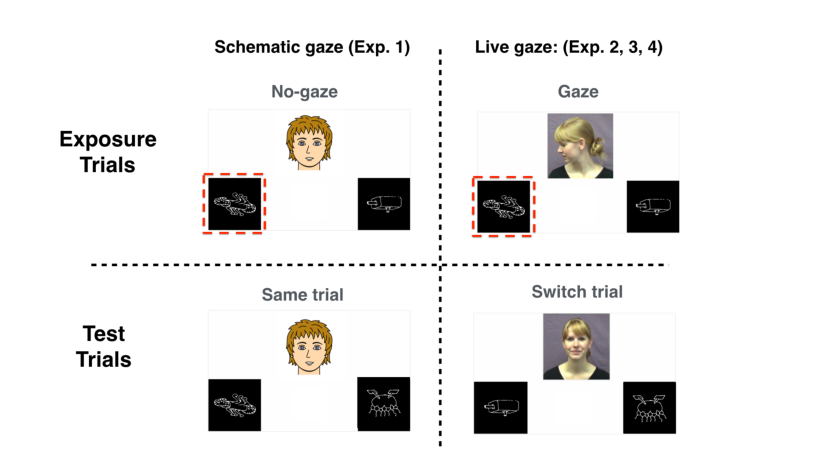
\includegraphics{figs/stimuli-1} \caption[Screenshots of exposure and test trials from Experiment 1 (schematic gaze cue) and Experiments 2 \& 3 (human actress gaze cue)]{%%%
\DIFdelendFL \DIFaddbeginFL 

{\centering 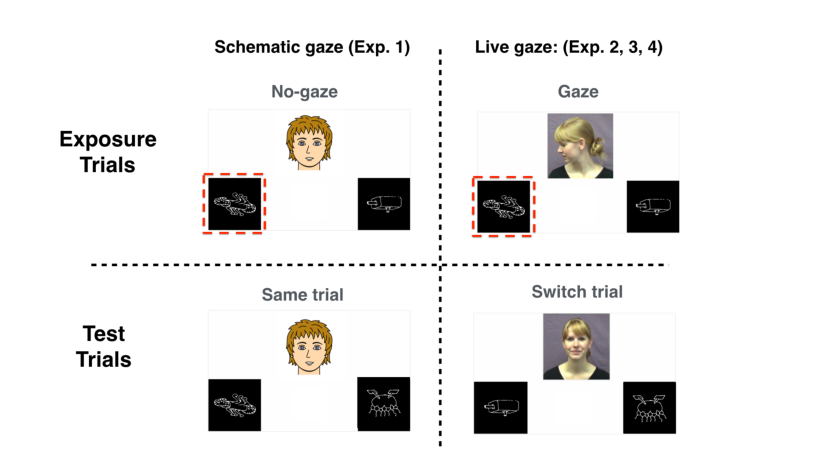
\includegraphics[width=1\linewidth]{figs/stimuli-1} 

}

\caption[Screenshots of exposure and test trials from Experiment 1 (schematic gaze cue) and Experiments 2, 3 \& 4 (live actress gaze cue)]{\DIFaddendFL Screenshots of exposure and test trials from Experiment 1 (schematic gaze cue) and Experiments 2\DIFdelbeginFL \DIFdelFL{\& }\DIFdelendFL \DIFaddbeginFL \DIFaddFL{, }\DIFaddendFL 3 \DIFaddbeginFL \DIFaddFL{\& 4 }\DIFaddendFL (\DIFdelbeginFL \DIFdelFL{human }\DIFdelendFL \DIFaddbeginFL \DIFaddFL{live }\DIFaddendFL actress gaze cue). Participants saw exposure trials with or without a gaze cue depending on condition assignment. All participants saw both types of test trials: Same and Switch. On Same trials\DIFaddbeginFL \DIFaddFL{, }\DIFaddendFL the object that participants chose during exposure appeared with a new novel object. On Switch trials the object that participants did not choose appeared with a new novel object.}\label{fig:stimuli}
\end{figure}
\end{CodeChunk}

\subsubsection{Stimuli}\label{stimuli}

Figure 1 shows screenshots taken from Experiment 1. Visual stimuli were
black and white pictures of familiar and novel objects taken from
Kanwisher, Woods, Iacoboni, \DIFdelbegin \DIFdel{\& }\DIFdelend \DIFaddbegin \DIFadd{and }\DIFaddend Mazziotta (1997). Auditory stimuli were
recordings of familiar and novel words by an AT\&T Natural Voices
\texttrademark (voice: Crystal) speech synthesizer. Novel words were 1-3
syllable pseudowords that obeyed all rules of English phonotactics. A
schematic drawing of a human speaker was chosen for ease of manipulating
the direction of gaze, the referential cue of interest in this study.
All experiments can be viewed and downloaded at the project page:
\url{https://kemacdonald.github.io/soc_xsit/}.

\subsubsection{Design and Procedure}\label{design-and-procedure}

Participants saw a total of 16 trials: eight exposure trials and eight
test trials. On each trial, they heard one novel word, saw a set of
novel objects, and were asked to guess which object went with the word.
Before seeing exposure and test trials, participants completed four
practice trials with familiar words and objects. These trials
familiarized participants to the task and allowed us to exclude
participants who were unlikely to perform the task as directed either
because of inattention or because their computer audio was turned off.

After the practice trials, participants were told that they would now
hear novel words and see novel objects \DIFdelbegin \DIFdel{, }\DIFdelend and that their task was to select
the referent that ``goes with each word.'' Over the course of the
experiment, participants heard eight novel words two times, with one
exposure trial and one test trial for each word. Four of the test trials
were \emph{Same} trials in which the object that participants selected
on the exposure trial was shown with a set of new novel objects. The
other four test trials were \emph{Switch} trials in which one of the
objects was chosen at random from the set of objects that the
participant did not select on exposure.

Participants were randomly assigned to \DIFaddbegin \DIFadd{one of }\DIFaddend the 32 between-subjects
conditions (4 Referents X 4 Intervals X 2 Gaze \DIFaddbegin \DIFadd{conditions}\DIFaddend ). Participants
either saw 2, 4, 6, or 8 referents on the screen and test trials
occurred \DIFdelbegin \DIFdel{after
}\DIFdelend \DIFaddbegin \DIFadd{at different intervals after exposure trials: }\DIFaddend either 0, 1, 3,
or 7 trials from the initial exposure to a word. \DIFaddbegin \DIFadd{For example, in the
0-interval condition, the test trial for that word would occur
immediately following the exposure trial, but in the 3-interval
condition, participants would see three additional exposure trials for
other novel words before seeing the test trial for the initial word. The
interval conditions modulated the time delay between learning and test,
and the number of referents conditions modulated the attention demands
present during learning.
}

\DIFaddend Participants were assigned to \DIFaddbegin \DIFadd{either }\DIFaddend the Gaze or \DIFdelbegin \DIFdel{No-gaze conditions}\DIFdelend \DIFaddbegin \DIFadd{No-Gaze condition}\DIFaddend . In
the Gaze condition, gaze was directed towards one of the objects on
exposure trials; in the \DIFdelbegin \DIFdel{No-gaze }\DIFdelend \DIFaddbegin \DIFadd{No-Gaze }\DIFaddend condition, gaze was always directed
straight ahead (see Figure 1 for examples\DIFdelbegin \DIFdel{of these trial types}\DIFdelend ). At test, gaze was \DIFdelbegin \DIFdel{never informative}\DIFdelend \DIFaddbegin \DIFadd{always
directed straight ahead}\DIFaddend . To show participants that their response had
been recorded, a red box appeared around the selected object for one
second. This box always appeared around the selected object, even if
participants' selections were incorrect.

\subsection{Results and Discussion}\label{results-and-discussion}

\subsubsection{Analysis plan}\label{analysis-plan}

The structure of our analysis plan is parallel across all \DIFdelbegin \DIFdel{three
}\DIFdelend \DIFaddbegin \DIFadd{four
}\DIFaddend experiments. First, we \DIFdelbegin \DIFdel{examine performance on Exposure }\DIFdelend \DIFaddbegin \DIFadd{examined accuracy and response time on exposure
}\DIFaddend trials to provide evidence that learners were (a) sensitive to our
experimental manipulation and (b) altered their allocation of attention
in response to \DIFdelbegin \DIFdel{changes in contextual ambiguity. Then we examine performance on
Test
trials to show that }\DIFdelend \DIFaddbegin \DIFadd{the presence of a social cue. Accuracy on exposure trials
was defined as selecting the referent that was the target of gaze in the
Gaze condition. (Note that there was no ``correct'' behavior for
exposure trials in the No-Gaze condition.) Next, we examined accuracy on
test trials to test whether }\DIFaddend learners' memory for alternative word-object
links \DIFdelbegin \DIFdel{changes }\DIFdelend \DIFaddbegin \DIFadd{changed }\DIFaddend depending on the ambiguity of the learning context.
\DIFaddbegin \DIFadd{Accuracy on test trials (both Same and Switch) was defined as selecting
the referent that was present during the exposure trial for that word.
}

\DIFaddend The key behavioral prediction of our hypothesis is that the presence of
gaze \DIFdelbegin \DIFdel{will }\DIFdelend \DIFaddbegin \DIFadd{would }\DIFaddend result in reduced memory for multiple word-object links,
operationalized as a decrease in \DIFdelbegin \DIFdel{performance }\DIFdelend \DIFaddbegin \DIFadd{accuracy }\DIFaddend on Switch test trials after
seeing \DIFdelbegin \DIFdel{Exposure }\DIFdelend \DIFaddbegin \DIFadd{exposure }\DIFaddend trials with a gaze cue. To quantify participants'
behavior, we \DIFdelbegin \DIFdel{use mixed effects }\DIFdelend \DIFaddbegin \DIFadd{used mixed-effects }\DIFaddend regression models with the maximal
random effects structure justified by our experimental design:
by-subject intercepts and slopes for each trial type. \DIFdelbegin \DIFdel{All mixed-effects }\DIFdelend \DIFaddbegin \DIFadd{We limited all
models to include only two-way interactions because the critical test of
our hypothesis was the interaction between gaze condition and trial
type, and we did not have theoretical predictions for any possible
three-way or four-way interactions. All }\DIFaddend models were fit using the lme4
package in R (Bates, Maechler, Bolker, \& Walker, 2013), and all of our
data \DIFdelbegin \DIFdel{, processing, and }\DIFdelend \DIFaddbegin \DIFadd{and our processing/}\DIFaddend analysis code can be viewed in the version
control repository for this paper at
\DIFdelbegin \DIFdel{:
}\DIFdelend \url{https://github.com/kemacdonald/soc_xsit}.

\begin{CodeChunk}
\begin{figure}[tb]
\DIFdelbeginFL %DIFDELCMD < 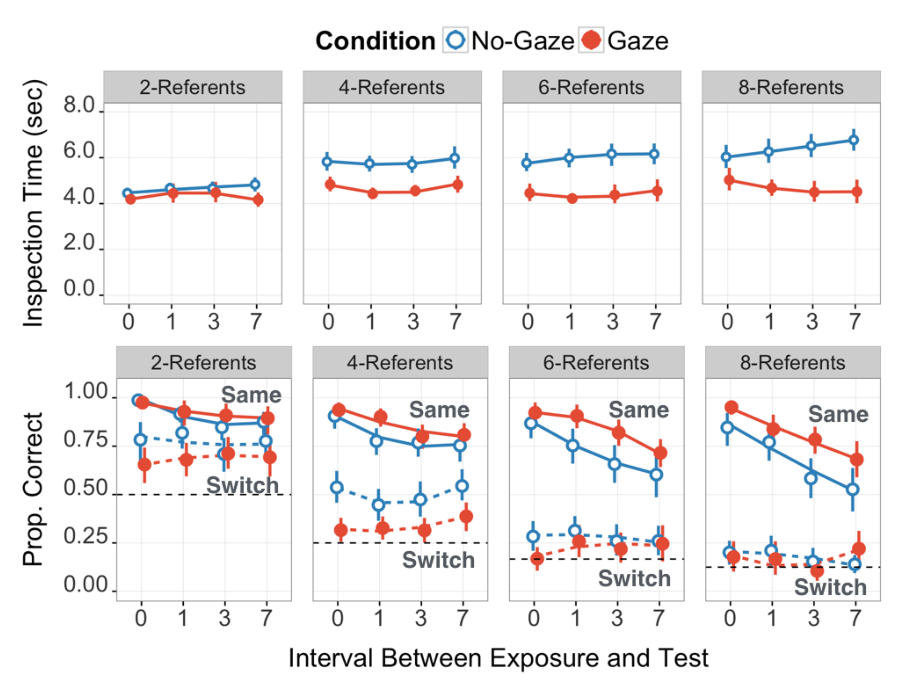
\includegraphics{figs/expt1-plot-1} %%%
\DIFdelendFL \DIFaddbeginFL 

{\centering 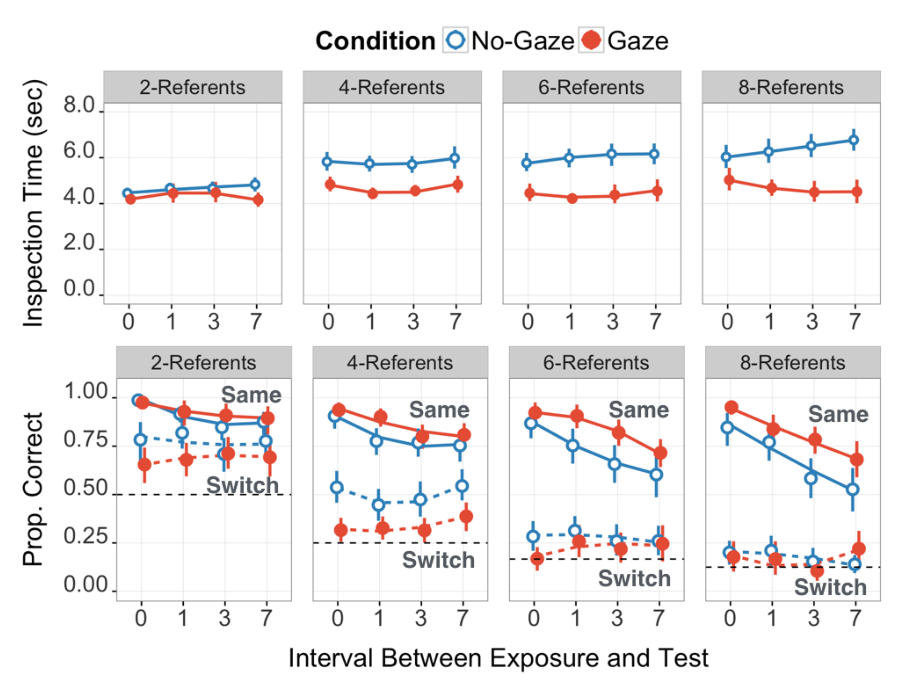
\includegraphics[width=1\linewidth]{figs/expt1-plot-1} 

}

\DIFaddendFL \caption[Experiment 1 results]{Experiment 1 results. \DIFdelbeginFL \DIFdelFL{Panel A }\DIFdelendFL \DIFaddbeginFL \DIFaddFL{The top row }\DIFaddendFL shows \DIFdelbeginFL \DIFdelFL{response }\DIFdelendFL \DIFaddbeginFL \DIFaddFL{average inspection }\DIFaddendFL times on exposure trials \DIFdelbeginFL \DIFdelFL{across }\DIFdelendFL \DIFaddbeginFL \DIFaddFL{for }\DIFaddendFL all experimental conditions \DIFdelbeginFL \DIFdelFL{: Gaze }\DIFdelendFL \DIFaddbeginFL \DIFaddFL{as a function of the number of trials that occurred between exposure }\DIFaddendFL and \DIFdelbeginFL \DIFdelFL{No-gaze}\DIFdelendFL \DIFaddbeginFL \DIFaddFL{test. Each panel represents a different number of referents}\DIFaddendFL , \DIFdelbeginFL \DIFdelFL{Referents (2, 4, 6, }\DIFdelendFL and \DIFdelbeginFL \DIFdelFL{8), }\DIFdelendFL \DIFaddbeginFL \DIFaddFL{line color represents the Gaze }\DIFaddendFL and \DIFdelbeginFL \DIFdelFL{Intervening trials (0, 1, 3, and 7)}\DIFdelendFL \DIFaddbeginFL \DIFaddFL{No-Gaze conditions}\DIFaddendFL . \DIFdelbeginFL \DIFdelFL{Panel B }\DIFdelendFL \DIFaddbeginFL \DIFaddFL{The bottom row }\DIFaddendFL shows accuracy on test trials for \DIFdelbeginFL \DIFdelFL{Same and Switch trials across }\DIFdelendFL all conditions \DIFaddbeginFL \DIFaddFL{as a function of the number of intervening trials}\DIFaddendFL . The horizontal dashed lines represent chance performance for each \DIFdelbeginFL \DIFdelFL{condition. Colored lines are linear model fits }\DIFdelendFL \DIFaddbeginFL \DIFaddFL{number of referents, }\DIFaddendFL and \DIFdelbeginFL \DIFdelFL{error }\DIFdelendFL \DIFaddbeginFL \DIFaddFL{the type of line (solid vs. dashed) represents the different test trial types (Same vs. Switch). Error }\DIFaddendFL bars indicate 95\% confidence intervals computed by non-parametric bootstrap.}\label{fig:expt1-plot}
\end{figure}
\end{CodeChunk}

\subsubsection{Exposure trials}\label{exposure-trials}

To ensure that our referential cue manipulation was effective\DIFdelbegin \DIFdel{we compare
participant' s accuracy
}\footnote{\DIFdel{Correct performance is defined as selecting the object that was the target of the speaker's gaze.}}
%DIFAUXCMD
\addtocounter{footnote}{-1}%DIFAUXCMD
\DIFdel{on Exposure }\DIFdelend \DIFaddbegin \DIFadd{, we
compared participants' accuracies on exposure }\DIFaddend trials in the Gaze
condition to a model of random behavior defined as a Binomial
distribution with a probability of success \(\frac{1}{Num Referents}\).
\DIFdelbegin \DIFdel{Following Yurovsky \& }\DIFdelend \DIFaddbegin \DIFadd{Correct performance was defined as selecting the object that was the
target of the speaker's gaze. Following Yurovsky and }\DIFaddend Frank (2015), we
fit logistic regressions for each \DIFdelbegin \DIFdel{Gaze, Referent, and Interval }\DIFdelend \DIFaddbegin \DIFadd{gaze, referent, and interval
}\DIFaddend combination specified as
\texttt{\DIFdelbegin \DIFdel{Correct }\DIFdelend \DIFaddbegin \DIFadd{Gaze Target }\DIFaddend $\sim$ 1 + offset(logit(1/Referents))}. The offset
\DIFdelbegin \DIFdel{encodes }\DIFdelend \DIFaddbegin \DIFadd{encoded }\DIFaddend the chance probability of success given the number of referents,
and the coefficient for the intercept term shows on a log-odds scale how
much more likely participants \DIFdelbegin \DIFdel{are }\DIFdelend \DIFaddbegin \DIFadd{were }\DIFaddend to select the gaze target than would
be expected if participants were selecting randomly. In all conditions\DIFaddbegin \DIFadd{,
}\DIFaddend participants used gaze to select referents on \DIFdelbegin \DIFdel{Exposure
}\DIFdelend \DIFaddbegin \DIFadd{exposure }\DIFaddend trials more often
than expected by chance (smallest \(\beta\) = \DIFdelbegin \DIFdel{2.56}\DIFdelend \DIFaddbegin \DIFadd{1.4}\DIFaddend , z = \DIFdelbegin \DIFdel{10.71, p }\DIFdelend \DIFaddbegin \DIFadd{9.38, \(p\)
}\DIFaddend \textless{} .001). \DIFaddbegin \DIFadd{However, there was variability across conditions in
the mean proportion of gaze cue (overall \(M\) = 0.84, range:
0.77--0.93).
}\DIFaddend 

We were also interested in differences in participants' response times
across the experimental conditions. Since these trials were self-paced,
participants could choose how much time to spend \DIFdelbegin \DIFdel{studying }\DIFdelend \DIFaddbegin \DIFadd{inspecting }\DIFaddend the
referents on the screen, thus providing an index of participants'
attention. To quantify the effects of gaze, interval, and number of
referents, we fit a linear \DIFdelbegin \DIFdel{mixed effects model predicting participants' response }\DIFdelend \DIFaddbegin \DIFadd{mixed-effects model that predicted
participants' inspection }\DIFaddend times as follows:
\texttt{\DIFdelbegin \DIFdel{RT }\DIFdelend \DIFaddbegin \DIFadd{Log(Inspection time) }\DIFaddend $\sim$ Gaze \DIFdelbegin \DIFdel{Condition }\DIFdelend * Log(Interval) \DIFaddbegin \DIFadd{+ Gaze }\DIFaddend * Log(Referents) + (1 | subject)}.
We found a significant main effect of \DIFaddbegin \DIFadd{the number of }\DIFaddend referents (\(\beta\)
= \DIFdelbegin \DIFdel{806.89}\DIFdelend \DIFaddbegin \DIFadd{0.34}\DIFaddend , p \textless{} .001) with \DIFdelbegin \DIFdel{slower responses }\DIFdelend \DIFaddbegin \DIFadd{longer inspection times }\DIFaddend as the number
of referents increased, \DIFdelbegin \DIFdel{and a significant two-way interaction between Gaze condition
and }\DIFdelend \DIFaddbegin \DIFadd{a significant interaction between gaze condition
and the }\DIFaddend number of referents (\(\beta\) = \DIFdelbegin \DIFdel{-517.36}\DIFdelend \DIFaddbegin \DIFadd{-0.27}\DIFaddend , p \textless{} .001) \DIFdelbegin \DIFdel{such
that responses were faster in the Gaze }\DIFdelend \DIFaddbegin \DIFadd{with
longer inspection times in the No-Gaze }\DIFaddend condition, especially as the
number of referents increased\DIFdelbegin \DIFdel{. The interaction between
Gaze condition and number of referents is shown in Panel A of Figure 2. Faster response
times on Exposure }\DIFdelend \DIFaddbegin \DIFadd{, and a significant interaction between
gaze condition and interval (\(\beta\) = -0.08, \(p\) = 0.004) with
slower inspection times in the No-Gaze condition, especially as the
number of intervening trials increased (see the top row of Figure 2).
Shorter inspection times on exposure }\DIFaddend trials with gaze provides \DIFdelbegin \DIFdel{preliminary }\DIFdelend evidence
that the presence of a referential cue focused participants' attention
on \DIFdelbegin \DIFdel{the
gaze target }\DIFdelend \DIFaddbegin \DIFadd{a single referent }\DIFaddend and away from alternative word-object links.

\subsubsection{Test trials}\label{test-trials}

\DIFdelbegin \DIFdel{Panel B of Figure 2 shows participants' accuracies }\DIFdelend \DIFaddbegin \DIFadd{Next, we explored participants' accuracy }\DIFaddend in identifying the referent for
each word in all conditions for both kinds of \DIFdelbegin \DIFdel{trials (Same
and Switch}\DIFdelend \DIFaddbegin \DIFadd{test trials (see the
bottom row of Figure 2}\DIFaddend ). We first compared the distribution of correct
responses made by each participant to the distribution expected if
participants were selecting randomly defined as a Binomial distribution
with a probability of success \(\frac{1}{Num Referents}\). \DIFaddbegin \DIFadd{Correct
performance is defined as selecting the object that was present on the
exposure trial for that word. }\DIFaddend We fit the same logistic regressions as we
did for \DIFdelbegin \DIFdel{Exposure }\DIFdelend \DIFaddbegin \DIFadd{exposure }\DIFaddend trials:
\texttt{Correct $\sim$ 1 + offset(logit(1/Referents))}. \DIFdelbegin \DIFdel{On }\DIFdelend \DIFaddbegin \DIFadd{In }\DIFaddend 31 out of the
32 conditions for both Same and Switch trials, participants chose the
correct \DIFdelbegin \DIFdel{target }\DIFdelend \DIFaddbegin \DIFadd{object }\DIFaddend more often than would be expected by chance (smallest
\(\beta\) = \DIFdelbegin \DIFdel{0.32, z }\DIFdelend \DIFaddbegin \DIFadd{0.36, \(z\) }\DIFaddend = \DIFdelbegin \DIFdel{1.96, p }\DIFdelend \DIFaddbegin \DIFadd{2.44, \(p\) }\DIFaddend = \DIFdelbegin \DIFdel{0.05}\DIFdelend \DIFaddbegin \DIFadd{0.01}\DIFaddend ). On Switch trials in the
\DIFdelbegin \DIFdel{8
referent, 3 interval }\DIFdelend \DIFaddbegin \DIFadd{8-referent, 3-interval }\DIFaddend condition, participants' responses were not
significantly different from chance (\(\beta\) = \DIFdelbegin \DIFdel{0.09}\DIFdelend \DIFaddbegin \DIFadd{0.06}\DIFaddend , z = \DIFdelbegin \DIFdel{0.5, p }\DIFdelend \DIFaddbegin \DIFadd{0.33, \(p\) }\DIFaddend =
\DIFdelbegin \DIFdel{0.62}\DIFdelend \DIFaddbegin \DIFadd{0.74}\DIFaddend ). Participants' success on Switch trials replicates the findings
from Yurovsky \DIFdelbegin \DIFdel{\& }\DIFdelend \DIFaddbegin \DIFadd{and }\DIFaddend Frank (2015) and provides direct evidence that
learners \DIFdelbegin \DIFdel{encoded }\DIFdelend \DIFaddbegin \DIFadd{encode }\DIFaddend more than a single hypothesis in ambiguous word learning
situations \DIFdelbegin \DIFdel{, }\DIFdelend even under high attentional and memory demands \DIFdelbegin \DIFdel{, and even }\DIFdelend \DIFaddbegin \DIFadd{and }\DIFaddend in the
presence of a referential cue.

\begin{table}[tb]
\centering
\begin{tabular}{lrrrrl}
 Predictor & Estimate & Std. Error & $z$ value & $p$ value &  \\ 
  \hline
Intercept & \DIFdelbeginFL \DIFdelFL{2.93 }\DIFdelendFL \DIFaddbeginFL \DIFaddFL{3.01 }\DIFaddendFL & \DIFdelbeginFL \DIFdelFL{0.28 }\DIFdelendFL \DIFaddbeginFL \DIFaddFL{0.29 }\DIFaddendFL & \DIFdelbeginFL \DIFdelFL{10.28 }\DIFdelendFL \DIFaddbeginFL \DIFaddFL{10.35 }\DIFaddendFL & $<$ .001 & *** \\ 
  Switch Trial & \DIFdelbeginFL \DIFdelFL{-1.37 }\DIFdelendFL \DIFaddbeginFL \DIFaddFL{-1.36 }\DIFaddendFL & \DIFdelbeginFL \DIFdelFL{0.23 }\DIFdelendFL \DIFaddbeginFL \DIFaddFL{0.24 }\DIFaddendFL & \DIFdelbeginFL \DIFdelFL{-5.90 }\DIFdelendFL \DIFaddbeginFL \DIFaddFL{-5.63 }\DIFaddendFL & $<$ .001 & *** \\ 
  Gaze Condition & \DIFdelbeginFL \DIFdelFL{-0.37 }\DIFdelendFL \DIFaddbeginFL \DIFaddFL{0.12 }\DIFaddendFL & \DIFdelbeginFL \DIFdelFL{0.25 }\DIFdelendFL \DIFaddbeginFL \DIFaddFL{0.26 }\DIFaddendFL & \DIFdelbeginFL \DIFdelFL{-1.48 }\DIFdelendFL \DIFaddbeginFL \DIFaddFL{0.47 }\DIFaddendFL & \DIFdelbeginFL \DIFdelFL{0.14 }\DIFdelendFL \DIFaddbeginFL \DIFaddFL{0.64 }\DIFaddendFL &  \\ 
  Log(Interval) & \DIFdelbeginFL \DIFdelFL{-0.42 }\DIFdelendFL \DIFaddbeginFL \DIFaddFL{-0.45 }\DIFaddendFL & 0.11 & \DIFdelbeginFL \DIFdelFL{-3.88 }\DIFdelendFL \DIFaddbeginFL \DIFaddFL{-4.08 }\DIFaddendFL & $<$ .001 & *** \\ 
  Log(Referents) & \DIFdelbeginFL \DIFdelFL{0.31 }\DIFdelendFL \DIFaddbeginFL \DIFaddFL{0.23 }\DIFaddendFL & 0.11 & \DIFdelbeginFL \DIFdelFL{2.73 }\DIFdelendFL \DIFaddbeginFL \DIFaddFL{2.02 }\DIFaddendFL & \DIFdelbeginFL \DIFdelFL{0.01 }\DIFdelendFL \DIFaddbeginFL \DIFaddFL{0.04 }\DIFaddendFL & \DIFdelbeginFL \DIFdelFL{** }\DIFdelendFL \DIFaddbeginFL \DIFaddFL{* }\DIFaddendFL \\ 
  Switch Trial*Gaze Condition & \DIFdelbeginFL \DIFdelFL{-0.81 }\DIFdelendFL \DIFaddbeginFL \DIFaddFL{-1.09 }\DIFaddendFL & 0.12 & \DIFdelbeginFL \DIFdelFL{-6.77 }\DIFdelendFL \DIFaddbeginFL \DIFaddFL{-9.07 }\DIFaddendFL & $<$ .001 & *** \\ 
  Switch Trial*Log(Interval) & 0.52 & 0.05 & \DIFdelbeginFL \DIFdelFL{9.53 }\DIFdelendFL \DIFaddbeginFL \DIFaddFL{9.50 }\DIFaddendFL & $<$ .001 & *** \\ 
  Switch Trial*Log(Referent) & \DIFdelbeginFL \DIFdelFL{-0.60 }\DIFdelendFL \DIFaddbeginFL \DIFaddFL{-0.59 }\DIFaddendFL & 0.09 & \DIFdelbeginFL \DIFdelFL{-6.94 }\DIFdelendFL \DIFaddbeginFL \DIFaddFL{-6.49 }\DIFaddendFL & $<$ .001 & *** \\ 
  Gaze Condition*Log(Interval) & \DIFdelbeginFL \DIFdelFL{0.02 }\DIFdelendFL \DIFaddbeginFL \DIFaddFL{0.06 }\DIFaddendFL & 0.06 & \DIFdelbeginFL \DIFdelFL{0.31 }\DIFdelendFL \DIFaddbeginFL \DIFaddFL{1.00 }\DIFaddendFL & \DIFdelbeginFL \DIFdelFL{0.76 }\DIFdelendFL \DIFaddbeginFL \DIFaddFL{0.32 }\DIFaddendFL &  \\ 
  Gaze Condition*Log(Referent) & \DIFdelbeginFL \DIFdelFL{0.26 }\DIFdelendFL \DIFaddbeginFL \DIFaddFL{0.20 }\DIFaddendFL & 0.09 & \DIFdelbeginFL \DIFdelFL{2.79 }\DIFdelendFL \DIFaddbeginFL \DIFaddFL{2.15 }\DIFaddendFL & \DIFdelbeginFL \DIFdelFL{0.01 }\DIFdelendFL \DIFaddbeginFL \DIFaddFL{0.03 }\DIFaddendFL & \DIFdelbeginFL \DIFdelFL{** }\DIFdelendFL \DIFaddbeginFL \DIFaddFL{* }\DIFaddendFL \\ 
  Log(Interval)*Log(Referent) & \DIFdelbeginFL \DIFdelFL{-0.06 }\DIFdelendFL \DIFaddbeginFL \DIFaddFL{-0.04 }\DIFaddendFL & 0.04 & \DIFdelbeginFL \DIFdelFL{-1.42 }\DIFdelendFL \DIFaddbeginFL \DIFaddFL{-1.02 }\DIFaddendFL & \DIFdelbeginFL \DIFdelFL{0.15 }\DIFdelendFL \DIFaddbeginFL \DIFaddFL{0.31 }\DIFaddendFL &  \\ 
   \hline
\end{tabular}
\caption{Predictor estimates with standard errors and significance information for a logistic mixed-effects model predicting word learning in Experiment 1.} 
\label{tab:exp1_reg}
\end{table}

To quantify the \DIFdelbegin \DIFdel{effect of each predictor }\DIFdelend \DIFaddbegin \DIFadd{effects of gaze, interval, and number of referents }\DIFaddend on
the probability of a correct response, we fit the following
mixed-effects logistic regression model to a filtered dataset \DIFdelbegin \DIFdel{, removing participants who were not reliably selecting the referent }\DIFdelend \DIFaddbegin \DIFadd{where we
removed participants who did not reliably select the object }\DIFaddend that was the
target of gaze on exposure trials:\footnote{We did not predict that
  there would be a subset of participants who would not follow the gaze
  cue, thus this filtering criteria was developed \DIFdelbegin \DIFdel{post-hoc}\DIFdelend \DIFaddbegin \DIFadd{posthoc}\DIFaddend . However, we
  \DIFdelbegin \DIFdel{believe }\DIFdelend \DIFaddbegin \DIFadd{think that }\DIFaddend the filter is theoretically motivated because we would only
  expect to see an effect of gaze if participants \DIFdelbegin \DIFdel{were }\DIFdelend actually \DIFdelbegin \DIFdel{using }\DIFdelend \DIFaddbegin \DIFadd{used }\DIFaddend the gaze
  cue. The filter \DIFdelbegin \DIFdel{removes 90 }\DIFdelend \DIFaddbegin \DIFadd{removed 94 }\DIFaddend participants \DIFdelbegin \DIFdel{who did not reliably select }\DIFdelend \DIFaddbegin \DIFadd{(6\% of }\DIFaddend the \DIFdelbegin \DIFdel{gaze target on exposure trials}\DIFdelend \DIFaddbegin \DIFadd{sample)}\DIFaddend . The key
  inferences from the data do not depend on this filtering criteria.}
\texttt{Correct $\sim$ Trial Type * Gaze + Trial Type * Log(Interval) + Trial Type * \DIFaddbegin \\ \DIFaddend Log(Referents) + \DIFdelbegin %DIFDELCMD < \\ %%%
\DIFdelend offset(logit($^1/_{Referents}$)) + (TrialType | subject)}.
\DIFdelbegin \DIFdel{We follow Yurovsky \& Frank (2015)'s analysis plan and }\DIFdelend \DIFaddbegin 

\DIFadd{We }\DIFaddend coded interval and number of referents as continuous predictors and
transformed these variables to the log scale. We limited the model to
include only two-way interactions because the critical test of our
hypothesis is the interaction between \DIFdelbegin \DIFdel{Gaze condition and Trial Type}\DIFdelend \DIFaddbegin \DIFadd{gaze condition and trial type}\DIFaddend , and
we did not have any theoretical predictions for possible three-way
interactions.
\footnote{If we \DIFdelbegin \DIFdel{allow }\DIFdelend \DIFaddbegin \DIFadd{allowed }\DIFaddend for three-way interactions in the model, there \DIFdelbegin \DIFdel{is }\DIFdelend \DIFaddbegin \DIFadd{was }\DIFaddend a \DIFaddbegin \DIFadd{marginally }\DIFaddend significant interaction between \DIFdelbegin \DIFdel{Gaze }\DIFdelend \DIFaddbegin \DIFadd{gaze }\DIFaddend condition, \DIFdelbegin \DIFdel{Trial Type}\DIFdelend \DIFaddbegin \DIFadd{trial type}\DIFaddend , and \DIFdelbegin \DIFdel{Interval }\DIFdelend \DIFaddbegin \DIFadd{interval }\DIFaddend (\DIFdelbegin \DIFdel{$\beta = 0.31$}\DIFdelend \DIFaddbegin \DIFadd{$\beta = 0.21$}\DIFaddend , \DIFdelbegin \DIFdel{p $<$ .01}\DIFdelend \DIFaddbegin \DIFadd{$p$ = 0.058}\DIFaddend ). The two-way interaction between \DIFdelbegin \DIFdel{Gaze }\DIFdelend \DIFaddbegin \DIFadd{gaze }\DIFaddend condition and \DIFdelbegin \DIFdel{Trial Type remains }\DIFdelend \DIFaddbegin \DIFadd{trial type remained }\DIFaddend significant in this more complex model \DIFaddbegin \DIFadd{($\beta = -1.3$, $p$ = 0.006)}\DIFaddend . A model including four-way interactions did not sufficiently improve model fit in order to justify the added complexity.}

Table 1 shows the output of the logistic regression. We found
significant main effects of \DIFdelbegin \DIFdel{Referents (\(\beta = 0.31\),
p }\DIFdelend \DIFaddbegin \DIFadd{the number of referents (\(\beta = 0.23\),
\(p\) }\DIFaddend \textless{} .001) and \DIFdelbegin \DIFdel{Interval (\(\beta = -0.42\), p }\DIFdelend \DIFaddbegin \DIFadd{interval (\(\beta = -0.45\), \(p\)
}\DIFaddend \textless{} .001), such that as each of these factors increased,
accuracy on test trials decreased. We also found \DIFdelbegin \DIFdel{significant main effects of Trial Type (\(\beta = -1.37\), p
}\DIFdelend \DIFaddbegin \DIFadd{a significant main
effect of trial type (\(\beta = -1.36\), \(p\) }\DIFaddend \textless{} .001), with
worse \DIFdelbegin \DIFdel{overall }\DIFdelend performance on Switch trials. There were significant interactions
between \DIFdelbegin \DIFdel{Trial Type and Interval
}\DIFdelend \DIFaddbegin \DIFadd{trial type and interval }\DIFaddend (\(\beta = 0.52\), \DIFdelbegin \DIFdel{p }\DIFdelend \DIFaddbegin \DIFadd{\(p\) }\DIFaddend \textless{}
.001), \DIFdelbegin \DIFdel{Trial Type and Referents
(\(\beta = -0.6\), p }\DIFdelend \DIFaddbegin \DIFadd{trial type and referents (\(\beta = -0.59\), \(p\) }\DIFaddend \textless{}
.001), and \DIFdelbegin \DIFdel{Gaze condition and Referents
(\(\beta = 0.26\), p }\DIFdelend \DIFaddbegin \DIFadd{gaze condition and referents (\(\beta = 0.2\), \(p\)
}\DIFaddend \textless{} .05). These interactions can be interpreted as \DIFaddbegin \DIFadd{meaning: }\DIFaddend (a)
the interval between exposure and test \DIFdelbegin \DIFdel{affecting }\DIFdelend \DIFaddbegin \DIFadd{affected }\DIFaddend Same trials more than
Switch trials, (b) the number of referents \DIFdelbegin \DIFdel{affecting
}\DIFdelend \DIFaddbegin \DIFadd{affected }\DIFaddend Switch trials more
than Same trials, and (c) participants \DIFdelbegin \DIFdel{performing
}\DIFdelend \DIFaddbegin \DIFadd{performed }\DIFaddend slightly better at \DIFaddbegin \DIFadd{the
}\DIFaddend higher number of referents in the Gaze condition\DIFdelbegin \DIFdel{(see
Panel B of Figure 2)}\DIFdelend . The interactions
between \DIFdelbegin \DIFdel{Gaze condition and Referents and between Referents and Interval }\DIFdelend \DIFaddbegin \DIFadd{gaze condition and referents and between referents and interval
}\DIFaddend were not significant. \DIFdelbegin \DIFdel{Crucially}\DIFdelend \DIFaddbegin \DIFadd{Importantly}\DIFaddend , we found the predicted interaction
between \DIFdelbegin \DIFdel{Trial Type and Gaze condition (\(\beta = -0.81\), p }\DIFdelend \DIFaddbegin \DIFadd{trial type and gaze condition (\(\beta = -1.09\), \(p\)
}\DIFaddend \textless{} .001), with participants in the Gaze condition performing
worse on Switch trials. This interaction provides direct evidence that
the presence of a referential cue selectively \DIFdelbegin \DIFdel{reduced }\DIFdelend \DIFaddbegin \DIFadd{reduces }\DIFaddend participants'
memory for alternative word-object links.

\DIFaddbegin \DIFadd{We were also interested in how inspection times on exposure trials would
affect participants' accuracy at test. So we fit an additional model
where participants' inspection times were added as a predictor. We found
a significant interaction between inspection time and gaze condition
(\(\beta = -0.17\), \(p\) = 0.01), such that longer inspection times
provided a larger boost to accuracy in the No-Gaze condition. This
interaction suggests that the presence of a referential cue modulated
the relationship between attention on exposure trials and memory at
test. Importantly, the key test of our hypothesis, the interaction
between gaze condition and trial type, remained significant in this
alternative version of the model (\(\beta\) = -1.02, \(p\) = p
\textless{} .001).
}

\DIFaddend Taken together, the \DIFdelbegin \DIFdel{response }\DIFdelend \DIFaddbegin \DIFadd{inspection }\DIFaddend time and accuracy analyses provide
evidence that the presence of a referential cue modulated learners'
attention during learning, and in turn made them less likely to track
multiple word-object links. We did not see strong evidence that reduced
tracking of alternatives resulted in an increase in performance on Same
trials. This finding suggests that the limitations on Same trials may be
different than those regulating the distribution of attention on Switch
trials \DIFdelbegin \DIFdel{, }\DIFdelend since the presence of a referential cue selectively reduced
learners tracking of alternatives but apparently did not \DIFdelbegin \DIFdel{lead }\DIFdelend \DIFaddbegin \DIFadd{cause }\DIFaddend learners
to form a stronger memory of their single candidate hypothesis.

There was relatively large variation in performance across conditions in
group-level accuracy scores and in participants' tendency to \emph{use}
the referential cue on exposure trials. Moreover, we found a subset of
participants who did not reliably use the gaze cue at all, potentially
reducing the effect of gaze on cross-situational learning in this
experiment. It is possible that the effect of gaze was reduced because
the referential cue that we used -- a static schematic drawing of a
speaker -- was relatively weak compared to the cues present in
\DIFdelbegin \DIFdel{real
world }\DIFdelend \DIFaddbegin \DIFadd{real-world }\DIFaddend learning environments. \DIFdelbegin \DIFdel{We }\DIFdelend \DIFaddbegin \DIFadd{Thus we }\DIFaddend do not yet know how learners'
memory for alternatives during cross-situational learning would change
in the presence of a stronger and more ecologically valid referential
cue. \DIFaddbegin \DIFadd{We designed }\DIFaddend Experiment 2 \DIFdelbegin \DIFdel{attempts to answer }\DIFdelend \DIFaddbegin \DIFadd{to address }\DIFaddend this question.

\section{Experiment 2}\label{experiment-2}

In Experiment 2, we \DIFdelbegin \DIFdel{attempt }\DIFdelend \DIFaddbegin \DIFadd{set out }\DIFaddend to replicate the findings from Experiment 1
using a more ecologically valid stimulus set. We replaced the static,
schematic drawing with a video of a live actress. While \DIFdelbegin \DIFdel{the video
stimuli
is }\DIFdelend \DIFaddbegin \DIFadd{these stimuli
were }\DIFaddend still far from actual learning contexts, \DIFdelbegin \DIFdel{it }\DIFdelend \DIFaddbegin \DIFadd{they }\DIFaddend included a real
person who provided both a gaze cue and a head turn towards the target
object. To reduce the across-conditions variability \DIFaddbegin \DIFadd{that we found in
Experiment 1}\DIFaddend , we introduced a within-subjects design where each
participant saw both Gaze and \DIFdelbegin \DIFdel{No-gaze
exposure trials }\DIFdelend \DIFaddbegin \DIFadd{No-Gaze exposure trials in a blocked
design}\DIFaddend . We selected a subset of \DIFaddbegin \DIFadd{the }\DIFaddend conditions from Experiment 1 \DIFdelbegin \DIFdel{,
testing }\DIFdelend \DIFaddbegin \DIFadd{and
tested }\DIFaddend only the 4-referent display with 0 and 3 intervening trials as
between-subjects manipulations. Our goals were to replicate the
reduction in learners' \DIFdelbegin \DIFdel{multiple alternatives tracking }\DIFdelend \DIFaddbegin \DIFadd{tracking of alternative word-object links }\DIFaddend in the
presence of \DIFdelbegin \DIFdel{referential cues, }\DIFdelend \DIFaddbegin \DIFadd{a referential cue }\DIFaddend and to test whether increasing the
ecological validity of the cue would result in a boost to the strength
of learners' recall of their \DIFdelbegin \DIFdel{single }\DIFdelend candidate hypothesis.

\subsection{Method}\label{method-1}

\subsubsection{Participants}\label{participants-1}

Participant recruitment and inclusionary/exclusionary criteria were
identical to those of Experiment \DIFdelbegin \DIFdel{1 (excluded 36 HITs). }\DIFdelend \DIFaddbegin \DIFadd{1. }\DIFaddend 100 HITs were posted for each
condition (1 Referent X 2 Intervals X 2 Gaze conditions) for total of
400 paid HITs \DIFaddbegin \DIFadd{(excluded 33 HITs)}\DIFaddend .

\subsubsection{Stimuli}\label{stimuli-1}

Audio and picture stimuli were identical to Experiment 1. The
referential cue in the Gaze condition was a video (see Figure 1). On
each exposure trial, the actress looked out at the participant with a
neutral expression, smiled, and then turned to look at one of the four
images on the screen. She maintained her gaze for 3 seconds before
returning to the center. On test trials, she looked straight ahead for
the duration of the trial.

\subsection{Design and Procedure}\label{design-and-procedure-1}

Procedures were identical to those of Experiment 1. The major design
change was a within-subjects manipulation of the gaze cue \DIFdelbegin \DIFdel{with each
participant seeing }\DIFdelend \DIFaddbegin \DIFadd{where each
participant saw }\DIFaddend exposure trials with and without gaze. The experiment
consisted of 32 trials \DIFdelbegin \DIFdel{broken down }\DIFdelend \DIFaddbegin \DIFadd{split }\DIFaddend into 2 blocks of 16 trials. Each block
consisted of 8 exposure trials and 8 test trials (4 Same trials and 4
Switch trials) \DIFdelbegin \DIFdel{, }\DIFdelend and contained only Gaze or No-gaze exposure trials. The
order of block was counterbalanced across participants.

\subsection{Results and Discussion}\label{results-and-discussion-1}

We followed the same analysis plan as in Experiment \DIFdelbegin \DIFdel{1, first analyzing
performance }\DIFdelend \DIFaddbegin \DIFadd{1. We first analyzed
inspection times and accuracy }\DIFaddend on exposure trials \DIFdelbegin \DIFdel{, and then analyzing performance }\DIFdelend \DIFaddbegin \DIFadd{and then analyzed
accuracy }\DIFaddend on test trials.

\subsubsection{Exposure trials}\label{exposure-trials-1}

Similar to Experiment 1, participants' responses on exposure trials
differed from those expected by chance (smallest \(\beta\) = 3.42, z =
33.43, \DIFdelbegin \DIFdel{p }\DIFdelend \DIFaddbegin \DIFadd{\(p\) }\DIFaddend \textless{} .001), suggesting that gaze was effective in
directing \DIFdelbegin \DIFdel{attention to the target referent}\DIFdelend \DIFaddbegin \DIFadd{participants' attention}\DIFaddend . Participants in Experiment 2 were
\DIFdelbegin \DIFdel{numerically }\DIFdelend more consistent in their use of gaze with the live action stimuli
compared to the schematic stimuli used in Experiment 1 (\DIFdelbegin \DIFdel{\(M_1 = .76, M_2 = .81\)}\DIFdelend \DIFaddbegin \DIFadd{\(M_{Exp1}\) =
0.8, \(M_{Exp2}\) = 0.91\$}\DIFaddend ), suggesting that using a live actress
\DIFdelbegin \DIFdel{resulted in a slight increase in }\DIFdelend \DIFaddbegin \DIFadd{increased }\DIFaddend participants' willingness to \DIFdelbegin \DIFdel{follow }\DIFdelend \DIFaddbegin \DIFadd{use }\DIFaddend the gaze cue.

\DIFdelbegin \DIFdel{Panel A of Figure 3 shows participants' response times. We replicate }\DIFdelend \DIFaddbegin \DIFadd{We replicated }\DIFaddend the findings from Experiment \DIFdelbegin \DIFdel{1, with faster response times in Gaze
condition. We fit a linear mixed effects model to response times with
the same specification as Experiment 1, finding main effects for Gaze condition }\DIFdelend \DIFaddbegin \DIFadd{1. Inspection times were
shorter in the Gaze }\DIFaddend (\(\beta\) = \DIFdelbegin \DIFdel{-1112.83, p }\DIFdelend \DIFaddbegin \DIFadd{-1.11, \(p\) }\DIFaddend \textless{} .001) and \DIFdelbegin \DIFdel{Interval
}\DIFdelend \DIFaddbegin \DIFadd{the
3-interval condition }\DIFaddend (\(\beta\) = \DIFdelbegin \DIFdel{-498.96, p }\DIFdelend \DIFaddbegin \DIFadd{-0.5, \(p\) }\DIFaddend \textless{} .001)\DIFdelbegin \DIFdel{with faster responses in the
Gaze condition and in the longer Interval conditions. The
two-way
interaction between Gaze condition }\DIFdelend \DIFaddbegin \DIFadd{. The
interaction between gaze }\DIFaddend and interval was not significant, \DIFdelbegin \DIFdel{with gaze having }\DIFdelend \DIFaddbegin \DIFadd{meaning that
gaze had }\DIFaddend the same effect on participants' \DIFdelbegin \DIFdel{response }\DIFdelend \DIFaddbegin \DIFadd{inspection }\DIFaddend times at both
intervals \DIFaddbegin \DIFadd{(see Panel A of Figure 3)}\DIFaddend .

\begin{CodeChunk}
\begin{figure}[tb]
\DIFdelbeginFL %DIFDELCMD < 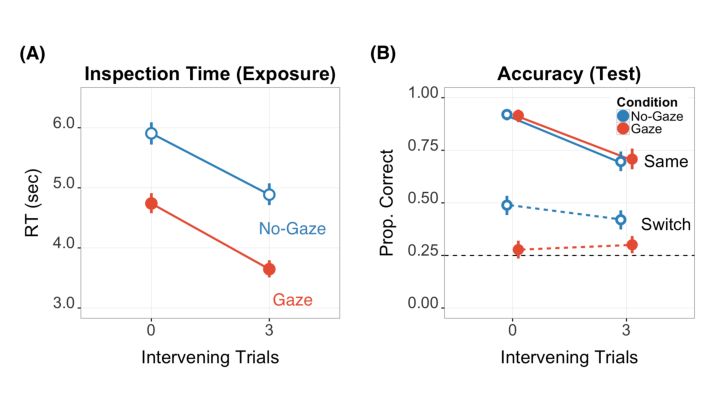
\includegraphics{figs/expt2-plot-1} %%%
\DIFdelendFL \DIFaddbeginFL 

{\centering 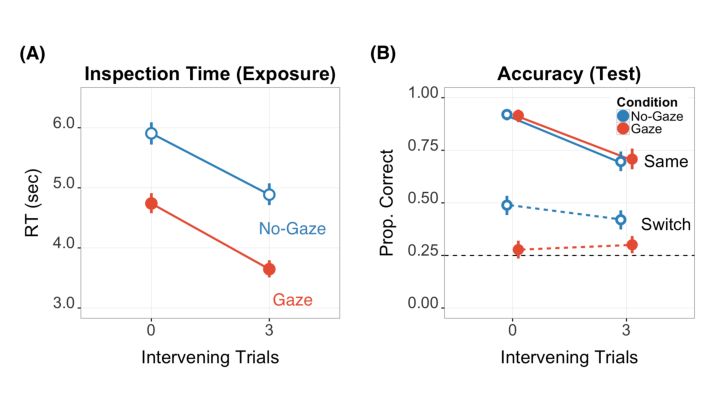
\includegraphics[width=1\linewidth]{figs/expt2-plot-1} 

}

\DIFaddendFL \caption[Experiment 2 results]{Experiment 2 results. Panel A shows \DIFdelbeginFL \DIFdelFL{study }\DIFdelendFL \DIFaddbeginFL \DIFaddFL{inspection }\DIFaddendFL times \DIFdelbeginFL \DIFdelFL{for }\DIFdelendFL \DIFaddbeginFL \DIFaddFL{on }\DIFaddendFL exposure trials with and without gaze. Panel B shows accuracy on \DIFdelbeginFL \DIFdelFL{test trials for same }\DIFdelendFL \DIFaddbeginFL \DIFaddFL{Same }\DIFaddendFL and Switch \DIFaddbeginFL \DIFaddFL{test }\DIFaddendFL trials\DIFdelbeginFL \DIFdelFL{across all conditions}\DIFdelendFL . \DIFdelbeginFL \DIFdelFL{The dashed line }\DIFdelendFL \DIFaddbeginFL \DIFaddFL{All plotting conventions are the same as }\DIFaddendFL in \DIFdelbeginFL \DIFdelFL{Panel B represents chance performance. }\DIFdelendFL \DIFaddbeginFL \DIFaddFL{Figure 2. }\DIFaddendFL Error bars indicate 95\% confidence intervals computed by non-parametric bootstrap.}\label{fig:expt2-plot}
\end{figure}
\end{CodeChunk}

\subsubsection{Test trials}\label{test-trials-1}

\begin{table}[tb]
\centering
\begin{tabular}{lrrrrl}
 Predictor & Estimate & Std. Error & $z$ value & $p$ value &  \\ 
  \hline
Intercept & \DIFdelbeginFL \DIFdelFL{2.69 }\DIFdelendFL \DIFaddbeginFL \DIFaddFL{2.98 }\DIFaddendFL & \DIFdelbeginFL \DIFdelFL{0.16 }\DIFdelendFL \DIFaddbeginFL \DIFaddFL{0.18 }\DIFaddendFL & \DIFdelbeginFL \DIFdelFL{16.84 }\DIFdelendFL \DIFaddbeginFL \DIFaddFL{16.20 }\DIFaddendFL & $<$ .001 & *** \\ 
  Switch Trial & \DIFdelbeginFL \DIFdelFL{-2.74 }\DIFdelendFL \DIFaddbeginFL \DIFaddFL{-3.04 }\DIFaddendFL & \DIFdelbeginFL \DIFdelFL{0.16 }\DIFdelendFL \DIFaddbeginFL \DIFaddFL{0.18 }\DIFaddendFL & \DIFdelbeginFL \DIFdelFL{-17.04 }\DIFdelendFL \DIFaddbeginFL \DIFaddFL{-16.47 }\DIFaddendFL & $<$ .001 & *** \\ 
  Gaze Condition & \DIFdelbeginFL \DIFdelFL{-0.12 }\DIFdelendFL \DIFaddbeginFL \DIFaddFL{-0.15 }\DIFaddendFL & 0.16 & \DIFdelbeginFL \DIFdelFL{-0.75 }\DIFdelendFL \DIFaddbeginFL \DIFaddFL{-0.98 }\DIFaddendFL & \DIFdelbeginFL \DIFdelFL{0.45 }\DIFdelendFL \DIFaddbeginFL \DIFaddFL{0.33 }\DIFaddendFL &  \\ 
  Log(Interval) & \DIFdelbeginFL \DIFdelFL{-0.88 }\DIFdelendFL \DIFaddbeginFL \DIFaddFL{-0.98 }\DIFaddendFL & \DIFdelbeginFL \DIFdelFL{0.09 }\DIFdelendFL \DIFaddbeginFL \DIFaddFL{0.10 }\DIFaddendFL & \DIFdelbeginFL \DIFdelFL{-9.40 }\DIFdelendFL \DIFaddbeginFL \DIFaddFL{-9.62 }\DIFaddendFL & $<$ .001 & *** \\ 
  Switch Trial*Gaze Condition & \DIFdelbeginFL \DIFdelFL{-0.73 }\DIFdelendFL \DIFaddbeginFL \DIFaddFL{-0.65 }\DIFaddendFL & 0.15 & \DIFdelbeginFL \DIFdelFL{-4.85 }\DIFdelendFL \DIFaddbeginFL \DIFaddFL{-4.32 }\DIFaddendFL & $<$ .001 & *** \\ 
  Switch Trial*Log(Interval) & \DIFdelbeginFL \DIFdelFL{0.76 }\DIFdelendFL \DIFaddbeginFL \DIFaddFL{0.85 }\DIFaddendFL & \DIFdelbeginFL \DIFdelFL{0.09 }\DIFdelendFL \DIFaddbeginFL \DIFaddFL{0.10 }\DIFaddendFL & \DIFdelbeginFL \DIFdelFL{8.35 }\DIFdelendFL \DIFaddbeginFL \DIFaddFL{8.68 }\DIFaddendFL & $<$ .001 & *** \\ 
  Gaze Condition*Log(Interval) & \DIFdelbeginFL \DIFdelFL{0.13 }\DIFdelendFL \DIFaddbeginFL \DIFaddFL{0.14 }\DIFaddendFL & 0.07 & \DIFdelbeginFL \DIFdelFL{1.81 }\DIFdelendFL \DIFaddbeginFL \DIFaddFL{1.90 }\DIFaddendFL & \DIFdelbeginFL \DIFdelFL{0.07 }\DIFdelendFL \DIFaddbeginFL \DIFaddFL{0.06 }\DIFaddendFL & . \\ 
   \hline
\end{tabular}
\caption{Predictor estimates with standard errors and significance information for a logistic mixed-effects model predicting word learning in Experiment 2.} 
\label{tab:exp2_reg}
\end{table}

\DIFdelbegin \DIFdel{Panel B of Figure 3 shows performance on test trials in Experiment 2.
}\DIFdelend Across all conditions for both \DIFdelbegin \DIFdel{Trial Types }\DIFdelend \DIFaddbegin \DIFadd{trial types }\DIFaddend participants selected the
correct referent at rates greater than chance (smallest \(\beta\) =
\DIFdelbegin \DIFdel{0.55}\DIFdelend \DIFaddbegin \DIFadd{0.58}\DIFaddend , z = \DIFdelbegin \DIFdel{9.04, p }\DIFdelend \DIFaddbegin \DIFadd{9.68, \(p\) }\DIFaddend \textless{} .001). We \DIFdelbegin \DIFdel{replicate }\DIFdelend \DIFaddbegin \DIFadd{replicated }\DIFaddend the critical
finding from Experiment 1: after seeing exposure trials with gaze,
participants performed worse on Switch trials, \DIFdelbegin \DIFdel{providing evidence that }\DIFdelend \DIFaddbegin \DIFadd{meaning }\DIFaddend they stored fewer
word-object links \DIFdelbegin \DIFdel{. We fit a mixed-effects logistic regression
model with the same specifications as in Experiment 1 and found
significant main effects of Interval (\(\beta = -0.88\), p }\DIFdelend \DIFaddbegin \DIFadd{(\(\beta = -0.65\), \(p\) }\DIFaddend \textless{}
.001)\DIFdelbegin \DIFdel{and Trial Type (\(\beta = -2.74\), p \textless{} .001).Participants were }\DIFdelend \DIFaddbegin \DIFadd{.}\footnote{\DIFadd{As in Experiment 1, we fit this model to a filtered dataset removing participants who did not reliably use the gaze cue.}}
\DIFadd{Participants were also }\DIFaddend less accurate as the interval between exposure
and test increased \DIFaddbegin \DIFadd{(\(\beta\) = -0.98, \(p\) \textless{} .001) }\DIFaddend and on
the Switch trials overall \DIFaddbegin \DIFadd{(\(\beta = -3.04\), \(p\) \textless{} .001)}\DIFaddend .

In addition, there was a significant \DIFdelbegin \DIFdel{two-way interaction between Trial
Type and
Interval (\(\beta = 0.76\), p }\DIFdelend \DIFaddbegin \DIFadd{interaction between trial type and
interval (\(\beta = 0.85\), \(p\) }\DIFaddend \textless{} .001), with worse
performance on Switch trials \DIFdelbegin \DIFdel{at the higher intervals, and a marginal
two-way interaction between Gaze condition and Interval
(\(\beta = 0.13\), p }\DIFdelend \DIFaddbegin \DIFadd{in the 3-interval condition. The
interaction between gaze condition and interval was marginally
significant (\(\beta = 0.14\), \(p\) }\DIFaddend = \DIFdelbegin \DIFdel{0.07)such that the number of intervening trials
had a smaller effect on participants ' performance in
the Gaze condition .
We found a robust interaction between Gaze condition and Trial Type
(\(\beta = -0.73\), p \textless{} .001) with Switch trials being more
difficult after gaze exposure
trials.}\footnote{\DIFdel{As in Experiment 1, we fit this model a filtered dataset removing participants who did not reliably use the gaze cue.}}
%DIFAUXCMD
\addtocounter{footnote}{-1}%DIFAUXCMD
\DIFdel{Once again, }\DIFdelend \DIFaddbegin \DIFadd{0.057), such that participants in
the gaze condition were less affected by the increase in interval.
Similar to Experiment 1, }\DIFaddend we did not see evidence of a boost to
performance on Same trials in the \DIFdelbegin \DIFdel{Gaze }\DIFdelend \DIFaddbegin \DIFadd{gaze }\DIFaddend condition.

\DIFaddbegin \DIFadd{Next, we added inspection times on exposure trials as a predictor of
accuracy at test. We found a marginally significant main effect of
inspection time (\(\beta\) = 0.18, \(p\) = 0.096) with higher accuracy
as inspection time increased. Similar to Experiment 1, the interaction
between gaze and trial type remained significant even when inspection
time was added to the model (\(\beta\) = -0.55, \(p\) \textless{} .001).
}

\DIFaddend The results of Experiment 2 provide converging evidence for our
hypothesis \DIFdelbegin \DIFdel{, showing }\DIFdelend that the presence of a referential cue reliably \DIFdelbegin \DIFdel{focused }\DIFdelend \DIFaddbegin \DIFadd{focuses
}\DIFaddend learners' attention away from alternative word-object links and \DIFdelbegin \DIFdel{shifted }\DIFdelend \DIFaddbegin \DIFadd{shifts
}\DIFaddend them towards single hypothesis tracking. \DIFdelbegin \DIFdel{Changing }\DIFdelend \DIFaddbegin \DIFadd{Moving }\DIFaddend to a live action
stimulus \DIFdelbegin \DIFdel{set led to slightly }\DIFdelend \DIFaddbegin \DIFadd{led to }\DIFaddend higher rates of selecting the target of gaze on exposure
trials, but did not result in a boost to performance on Same trials. The
selective effect of gaze on Switch trials provides additional evidence
that the fidelity of participants' single hypothesis was unaffected by
the presence of a referential cue in our paradigm.

Thus far we have shown that people store different amounts of
information in response to a categorical manipulation of referential
uncertainty. In both Experiments 1 and 2, the learning context was
either entirely ambiguous (\DIFdelbegin \DIFdel{No-gaze}\DIFdelend \DIFaddbegin \DIFadd{No-Gaze}\DIFaddend ) or entirely unambiguous (Gaze). But
not all \DIFdelbegin \DIFdel{real world }\DIFdelend \DIFaddbegin \DIFadd{real-world }\DIFaddend learning contexts fall at the extremes of this
continuum (although see Yurovsky et al., 2013). Could learners be
sensitive to more subtle changes in the quality of learning contexts? In
our next experiment, we \DIFdelbegin \DIFdel{test }\DIFdelend \DIFaddbegin \DIFadd{tested }\DIFaddend a prediction of our account: whether
learners \DIFaddbegin \DIFadd{would }\DIFaddend store more word-object links in response to graded
changes \DIFdelbegin \DIFdel{of
}\DIFdelend \DIFaddbegin \DIFadd{in }\DIFaddend referential uncertainty during learning.

\section{Experiment 3}\label{experiment-3}

In Experiment 3, we \DIFdelbegin \DIFdel{explore whether learners will }\DIFdelend \DIFaddbegin \DIFadd{explored whether learners would }\DIFaddend allocate attention
and memory flexibly in response to \emph{graded} changes in the
referential uncertainty \DIFaddbegin \DIFadd{that was }\DIFaddend present during learning. To test this
hypothesis, we \DIFdelbegin \DIFdel{move
}\DIFdelend \DIFaddbegin \DIFadd{moved }\DIFaddend beyond a categorical manipulation of the
presence/absence of gaze, and we parametrically \DIFdelbegin \DIFdel{vary }\DIFdelend \DIFaddbegin \DIFadd{varied }\DIFaddend the strength of
the referential cue. We \DIFdelbegin \DIFdel{manipulate }\DIFdelend \DIFaddbegin \DIFadd{manipulated }\DIFaddend cue strength by \DIFdelbegin \DIFdel{including }\DIFdelend \DIFaddbegin \DIFadd{adding }\DIFaddend a block of
familiarization trials where we \DIFdelbegin \DIFdel{vary }\DIFdelend \DIFaddbegin \DIFadd{varied }\DIFaddend the proportion of Same and Switch
trials. If participants saw more Switch trials, this \DIFdelbegin \DIFdel{provides }\DIFdelend \DIFaddbegin \DIFadd{provided }\DIFaddend evidence
that the speaker's gaze was \DIFdelbegin \DIFdel{an unreliable }\DIFdelend \DIFaddbegin \DIFadd{a less reliable }\DIFaddend cue to reference. This
design was inspired by a growing body of experimental work showing that
even young children are sensitive to the prior reliability of speakers
and will use this information \DIFdelbegin \DIFdel{when deciding }\DIFdelend \DIFaddbegin \DIFadd{to decide }\DIFaddend whom to learn novel words from
(Koenig, Clement, \& Harris, 2004).

\subsection{Method}\label{method-2}

\subsubsection{Participants}\label{participants-2}

Participant recruitment \DIFdelbegin \DIFdel{, }\DIFdelend and inclusionary/exclusionary criteria were
identical to those of Experiment 1 and 2 (excluded \DIFdelbegin \DIFdel{4 }\DIFdelend \DIFaddbegin \DIFadd{27 }\DIFaddend HITs). 100 HITs
were posted for each reliability level (0\%, 25\%, 50\%, 75\%, and
100\%) for total of 500 paid HITs.

\subsubsection{Design and Procedure}\label{design-and-procedure-2}

Procedures were identical to those of \DIFdelbegin \DIFdel{Experiment }\DIFdelend \DIFaddbegin \DIFadd{Experiments }\DIFaddend 1 and 2. We modified
\DIFaddbegin \DIFadd{the design of }\DIFaddend our cross-situational learning paradigm to include a block
of 16 familiarization trials (8 exposure trials and 8 test trials) \DIFdelbegin \DIFdel{, which
established the }\DIFdelend \DIFaddbegin \DIFadd{at
the beginning of the experiment. These trials served to establish the
}\DIFaddend reliability of the speaker\DIFaddbegin \DIFadd{'s gaze}\DIFaddend . To establish reliability, we varied
the proportion of Same/Switch trials that occurred during \DIFdelbegin \DIFdel{this
}\DIFdelend \DIFaddbegin \DIFadd{the
}\DIFaddend familiarization block. Recall that on Switch trials the gaze target \DIFdelbegin \DIFdel{does
}\DIFdelend \DIFaddbegin \DIFadd{did
}\DIFaddend not show up at test, \DIFdelbegin \DIFdel{thus providing evidence that this }\DIFdelend \DIFaddbegin \DIFadd{which provided evidence that the }\DIFaddend speaker's gaze \DIFdelbegin \DIFdel{might not be }\DIFdelend \DIFaddbegin \DIFadd{was
not }\DIFaddend a reliable cue to reference. \DIFdelbegin \DIFdel{Gaze reliability }\DIFdelend \DIFaddbegin \DIFadd{Reliability }\DIFaddend was a between-subjects
manipulation \DIFdelbegin \DIFdel{, with participants either seeing 0, 2}\DIFdelend \DIFaddbegin \DIFadd{such that participants either saw 8, 6}\DIFaddend , 4, \DIFdelbegin \DIFdel{6, or 8 Switch
trials }\DIFdelend \DIFaddbegin \DIFadd{2, or 0 Switch
trials during familiarization, which corresponded to the 0\%, 25\%,
50\%, 75\%, and 100\% reliability conditions}\DIFaddend . After the familiarization
block, participants completed another block of 16 trials (8 exposure
trials and 8 test trials). Since we were no longer testing the effect of
the presence or absence of a referential cue, all exposure trials
\DIFdelbegin \DIFdel{in Experiment 3
included gaze, but this cuewas more or less reliable depending on which
familiarization block participants saw}\DIFdelend \DIFaddbegin \DIFadd{throughout the experiment included a gaze cue}\DIFaddend . Finally, at the end of
the task\DIFaddbegin \DIFadd{, }\DIFaddend we asked participants to assess the reliability of the speaker
on a continuous scale from ``completely unreliable'' to ``completely
reliable.''

\subsection{Results and Discussion}\label{results-and-discussion-2}

\subsubsection{Exposure trials}\label{exposure-trials-2}

\DIFdelbegin \DIFdel{Similar to Experiments 1 and 2, participants }\DIFdelend \DIFaddbegin \DIFadd{Participants }\DIFaddend reliably chose the referent that was the target of gaze at
rates greater than \DIFdelbegin \DIFdel{those that would be
predicted by a guessing model }\DIFdelend \DIFaddbegin \DIFadd{chance }\DIFaddend (smallest \(\beta\) = \DIFdelbegin \DIFdel{2.57}\DIFdelend \DIFaddbegin \DIFadd{2.62}\DIFaddend , z = 33.43, \DIFdelbegin \DIFdel{p
}\DIFdelend \DIFaddbegin \DIFadd{\(p\)
}\DIFaddend \textless{} .001). \DIFdelbegin \DIFdel{To quantify the effect of reliability condition and
participants' subjective reliability assessment, we }\DIFdelend \DIFaddbegin \DIFadd{We }\DIFaddend fit a mixed effects logistic regression model
predicting the probability of selecting the gaze target as follows:
\texttt{Correct-Exposure $\sim$ Reliability Condition * Subjective Reliability + \DIFdelbegin \DIFdel{offset}\DIFdelend (\DIFdelbegin \DIFdel{logit(}\DIFdelend 1 \DIFdelbegin \DIFdel{/Referents)) + (1 }\DIFdelend | subject)}.
We found \DIFdelbegin \DIFdel{significant main effects of both }\DIFdelend \DIFaddbegin \DIFadd{an effect of }\DIFaddend reliability condition (\(\beta\) = \DIFdelbegin \DIFdel{3.3, p \textless{} .05) and }\DIFdelend \DIFaddbegin \DIFadd{3.28, \(p\) =
0.03) such that when the gaze cue was more reliable, participants were
more likely to use it (\(M_{0\%}\) = 0.83, \(M_{25\%}\) = 0.82,
\(M_{50\%}\) = 0.87, \(M_{75\%}\) = 0.9, \(M_{100\%}\) = 0.94). We also
found an effect of }\DIFaddend subjective reliability (\(\beta\) = \DIFdelbegin \DIFdel{7, p }\DIFdelend \DIFaddbegin \DIFadd{7.26, \(p\)
}\DIFaddend \textless{} .001) such that when \DIFaddbegin \DIFadd{participants thought }\DIFaddend the gaze cue was
\DIFdelbegin \DIFdel{more
reliableand when subjective reliability assessments were higher
participants were }\DIFdelend \DIFaddbegin \DIFadd{reliable, they were }\DIFaddend more likely to use \DIFdelbegin \DIFdel{the gaze cue}\DIFdelend \DIFaddbegin \DIFadd{it}\DIFaddend . The interaction between
\DIFdelbegin \DIFdel{speaker reliability }\DIFdelend \DIFaddbegin \DIFadd{reliability condition }\DIFaddend and subjective reliability assessments was
marginally significant (\(\beta\) = \DIFdelbegin \DIFdel{-4.33, p }\DIFdelend \DIFaddbegin \DIFadd{-4.58, \(p\)}\DIFaddend = \DIFdelbegin \DIFdel{0.1}\DIFdelend \DIFaddbegin \DIFadd{0.092}\DIFaddend ). This analysis
provides evidence that participants were sensitive to the reliability
manipulation both in how often they used the gaze cue \DIFdelbegin \DIFdel{during the task
}\DIFdelend and in how they
rated the \DIFaddbegin \DIFadd{reliability of the }\DIFaddend speaker at the end of the task.

\DIFaddbegin \subsubsection{\DIFadd{Test trials}}\label{test-trials-2}

\DIFaddend \begin{CodeChunk}
\begin{figure}[tb]
\DIFdelbeginFL %DIFDELCMD < 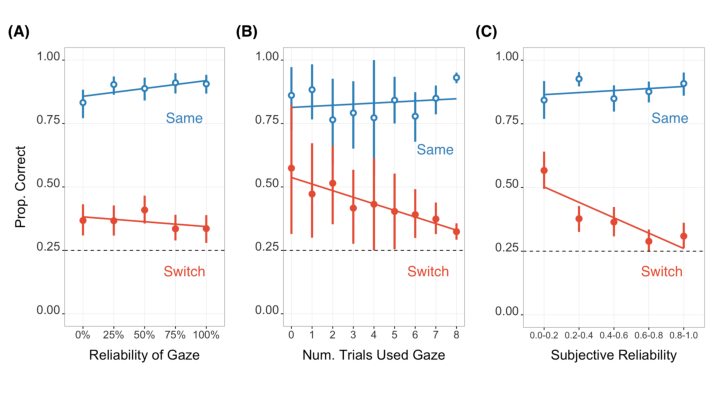
\includegraphics{figs/expt3-plot-1} \caption[Accuracy on test trials in Experiment 3 for both same and switch trial types]{%%%
\DIFdelFL{Accuracy on }\DIFdelendFL \DIFaddbeginFL 

{\centering 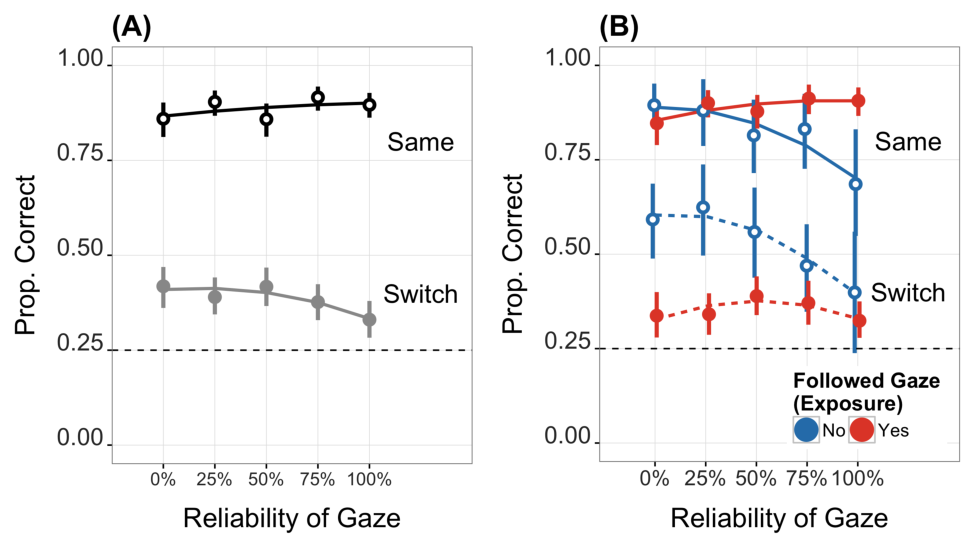
\includegraphics[width=0.9\linewidth]{figs/e3-plot-1} 

}

\caption[Primary analyses of test trial performance in Experiment 3]{\DIFaddFL{Primary analyses of }\DIFaddendFL test \DIFdelbeginFL \DIFdelFL{trials }\DIFdelendFL \DIFaddbeginFL \DIFaddFL{trial performance }\DIFaddendFL in Experiment \DIFdelbeginFL \DIFdelFL{3 for both same and switch trial types. }\DIFdelendFL \DIFaddbeginFL \DIFaddFL{3. }\DIFaddendFL Panel A shows \DIFdelbeginFL \DIFdelFL{accuracy }\DIFdelendFL \DIFaddbeginFL \DIFaddFL{performance }\DIFaddendFL as a function of \DIFdelbeginFL \DIFdelFL{the speaker's }\DIFdelendFL reliability \DIFaddbeginFL \DIFaddFL{condition}\DIFaddendFL . Panel B shows \DIFdelbeginFL \DIFdelFL{accuracy }\DIFdelendFL \DIFaddbeginFL \DIFaddFL{performance }\DIFaddendFL as a function of \DIFaddbeginFL \DIFaddFL{reliability condition and whether }\DIFaddendFL participants \DIFdelbeginFL \DIFdelFL{' }\DIFdelendFL \DIFaddbeginFL \DIFaddFL{chose to follow }\DIFaddendFL gaze \DIFdelbeginFL \DIFdelFL{following }\DIFdelendFL on exposure trials. \DIFdelbeginFL \DIFdelFL{Panel C shows accuracy as a function of participants' subjective reliability judgments, grouped into five equally spaced bins. }\DIFdelendFL The horizontal dashed \DIFdelbeginFL \DIFdelFL{line represents the expected performance if participants were selecting randomly. The colored }\DIFdelendFL lines \DIFdelbeginFL \DIFdelFL{are linear model fits }\DIFdelendFL \DIFaddbeginFL \DIFaddFL{represent chance performance, }\DIFaddendFL and error bars indicate 95\% confidence intervals computed by non-parametric bootstrap.}\DIFdelbeginFL %DIFDELCMD < \label{fig:expt3-plot}
%DIFDELCMD < %%%
\DIFdelendFL \DIFaddbeginFL \label{fig:e3-plot}
\DIFaddendFL \end{figure}
\end{CodeChunk}

\DIFdelbegin \subsubsection{\DIFdel{Test trials}}%DIFAUXCMD
\addtocounter{subsubsection}{-1}%DIFAUXCMD
%DIFDELCMD < \label{test-trials-2}
%DIFDELCMD < 

%DIFDELCMD < %%%
\DIFdel{Figure 4 shows performance on test trials in Experiment 3. }\DIFdelend \DIFaddbegin \DIFadd{Next, we tested whether the reliability manipulation altered the
strength of participants' memory for alternative word-object links.
}\DIFaddend Across all conditions\DIFdelbegin \DIFdel{for both Trial Types }\DIFdelend \DIFaddbegin \DIFadd{, }\DIFaddend participants selected the correct referent at
rates greater than chance (smallest \(\beta\) = \DIFdelbegin \DIFdel{0.41}\DIFdelend \DIFaddbegin \DIFadd{0.42}\DIFaddend , z = \DIFdelbegin \DIFdel{3.63, p }\DIFdelend \DIFaddbegin \DIFadd{3.69, \(p\)
}\DIFaddend \textless{} .001). Our primary prediction \DIFdelbegin \DIFdel{in this experiment is
}\DIFdelend \DIFaddbegin \DIFadd{was }\DIFaddend an interaction between
reliability and test trial type, with higher levels of reliability
leading to \DIFdelbegin \DIFdel{less attention and }\DIFdelend \DIFaddbegin \DIFadd{worse performance on Switch trials (i.e., less }\DIFaddend memory
allocated to alternative word-object links\DIFdelbegin \DIFdel{. To test }\DIFdelend \DIFaddbegin \DIFadd{). To explore }\DIFaddend this prediction,
we performed \DIFdelbegin \DIFdel{three complementary analysesof test trial performance using three
different predictors: reliability condition, participants' use of gaze,
and participants' subjective reliability assessment}\DIFdelend \DIFaddbegin \DIFadd{four complementary analyses: our primary analysis, which
tested the effect of the reliability manipulation, and three secondary
analyses, which explored the effects of participants' (a) use of the
gaze cue, (b) subjective reliability assessments, and (c) inspection
time on exposure trials}\DIFaddend .

\DIFaddbegin \begin{CodeChunk}
\begin{figure}[tb]

{\centering 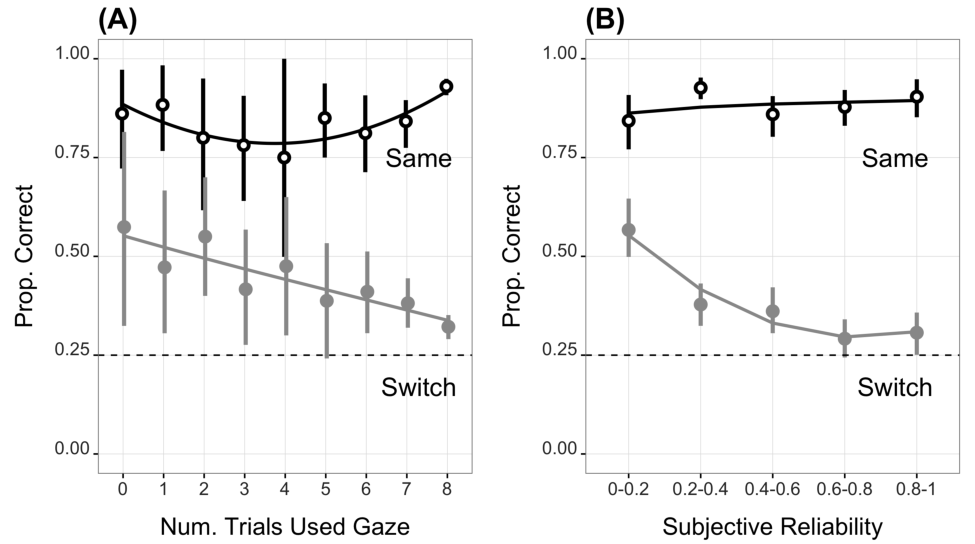
\includegraphics[width=0.9\linewidth]{figs/expt3-sub-plots-1} 

}

\caption[Secondary analyses of test trial performance in Experiment 3]{\DIFaddFL{Secondary analyses of test trial performance in Experiment 3. Panel A shows accuracy as a function of the number of exposure trials on which participants chose to use the gaze cue. Panel B shows accuracy as a function of participants' subjective reliability judgments. The horizontal dashed lines represent chance performance, and error bars indicate 95\% confidence intervals computed by non-parametric bootstrap.}}\label{fig:expt3-sub-plots}
\end{figure}
\end{CodeChunk}

\DIFaddend \paragraph{Reliability condition
analysis}\label{reliability-condition-analysis}

\DIFdelbegin \DIFdel{Panel A of Figure 4 shows participants' accuracy on both types of test trials as a function of the reliability manipulation. We fit a mixed-effects logistic regression }\DIFdelend \DIFaddbegin \DIFadd{To test the effect of reliability, we fit a }\DIFaddend model predicting accuracy \DIFaddbegin \DIFadd{at
test }\DIFaddend using reliability condition \DIFdelbegin \DIFdel{as a predictor and }\DIFdelend \DIFaddbegin \DIFadd{and test trial type as predictors. We
}\DIFaddend found a significant main effect of trial type (\DIFdelbegin \DIFdel{\(\beta = -1.85\), p }\DIFdelend \DIFaddbegin \DIFadd{\(\beta = -3.95\), \(p\)
}\DIFaddend \textless{} .001), with lower accuracy on Switch trials. We \DIFdelbegin \DIFdel{found a significant interaction between Reliability condition and Trial Type (\(\beta = -0.9\), p }\DIFdelend \DIFaddbegin \DIFadd{also found
the key interaction between reliability condition and trial type
(\(\beta\) }\DIFaddend = \DIFdelbegin \DIFdel{0.05), providing evidence for our key prediction. The interaction between
Reliability condition and accuracy was relatively weak, however, }\DIFdelend \DIFaddbegin \DIFadd{-0.76, \(p\) = 0.044), such that when gaze was more
reliable, participants performed worse on Switch trials (see Panel A of
Figure 4). This interaction suggests that people stored more word-object
links as the learning context becomes more ambiguous. However, the
interaction between reliability and trial type was not particularly
strong, }\DIFaddend and -- similar to Experiment 1 -- there was \DIFdelbegin \DIFdel{substantial variability }\DIFdelend \DIFaddbegin \DIFadd{variability in
performance }\DIFaddend across conditions (see the 50\% reliable condition in Panel
A of Figure 4). \DIFdelbegin \DIFdel{To
}\DIFdelend \DIFaddbegin \DIFadd{So to }\DIFaddend provide additional support for our hypothesis, we
conducted \DIFdelbegin \DIFdel{two
}\DIFdelend \DIFaddbegin \DIFadd{three }\DIFaddend follow-up analyses.

\paragraph{Gaze use \DIFdelbegin \DIFdel{analysis}\DIFdelend \DIFaddbegin \DIFadd{analyses}\DIFaddend }\DIFdelbegin %DIFDELCMD < \label{gaze-use-analysis}
%DIFDELCMD < %%%
\DIFdelend \DIFaddbegin \label{gaze-use-analyses}
\DIFaddend 

We would only expect to see a strong interaction between reliability and
trial type if learners chose to use the gaze cue during exposure trials.
To test this hypothesis, we fit \DIFdelbegin \DIFdel{a mixed effects logistic regression
modelwith the }\DIFdelend \DIFaddbegin \DIFadd{two additional models that included two
different measures of participants' use of the gaze cue. First, we added
accuracy on exposure trials as a predictor in our model. (Recall that
correct performance on exposure trials was defined as using the gaze
cue.) We found a significant interaction between accuracy on exposure
trials and trial type (\(\beta = -1.43\), \(p\) \textless{} .001) with
worse performance on Switch test trials when participants used gaze on
exposure trials (see Panel B of Figure 4). We also found an interaction
between gaze use and reliability (\(\beta = 0.97\), \(p\) = 0.004) such
that when gaze was more reliable, participants were more likely to use
it. The interaction between trial type and reliability became marginally
significant in this model (\(\beta = -0.62\), \(p\) = 0.086), suggesting
that participants' use of the gaze cue was a stronger predictor of
memory for alternative word-object links.}\footnote{\DIFadd{We are grateful to an
  anonymous reviewer for suggesting this analysis, but we would like to
  note that it is exploratory.}}

\DIFadd{We also hypothesized that the reliability manipulation might change how
often individual participants chose to use the gaze cue throughout the
task. To explore this possibility, we fit a model with the }\DIFaddend same
specifications, but \DIFdelbegin \DIFdel{substituting accuracy on exposure trials for reliability condition as a predictor}\DIFdelend \DIFaddbegin \DIFadd{we included a predictor that we created by binning
participants based on the number of exposure trials on which they chose
to follow gaze (i.e., a gaze following score)}\DIFaddend . We found a \DIFdelbegin \DIFdel{robust two-way interaction between accuracy }\DIFdelend \DIFaddbegin \DIFadd{significant
interaction between how often participants chose to follow gaze }\DIFaddend on
exposure trials and \DIFdelbegin \DIFdel{Trial
Type (\(\beta = -0.36\), p }\DIFdelend \DIFaddbegin \DIFadd{trial type (\(\beta = -0.32\), \(p\) }\DIFaddend \textless{}
.001)\DIFaddbegin \DIFadd{, }\DIFaddend such that participants who were more likely to use the gaze cue
performed worse on Switch trials, but not Same trials \DIFdelbegin \DIFdel{.}\footnote{\DIFdel{We found this interaction while performing
  exploratory data analysis on a previous version of this study with an
  independent sample (N = 250, \(\beta = -0.28\), p \textless{} .001).
  The results reported here are from a follow-up study where testing
  this interaction was a planned analysis.}} %DIFAUXCMD
\addtocounter{footnote}{-1}%DIFAUXCMD
\DIFdel{Panel B of
Figure 4 shows
this interaction.}\DIFdelend \DIFaddbegin \DIFadd{(see Panel A of
Figure 5).}\footnote{\DIFadd{We found this interaction while performing
  exploratory data analysis on a previous version of this study with an
  independent sample (N = 250, \(\beta = -0.29\), \(p\) \textless{}
  .001). The results reported here are from a follow-up study where
  testing this interaction was a planned analysis.}} \DIFadd{Taken together, the
two analyses of participants' use of the gaze cue provide converging
evidence that when the speaker's gaze was reliable participants were
more likely to use the cue, and when they followed gaze, they tended to
store less information from the initial naming event.
}\DIFaddend 

\paragraph{Subjective reliability
analysis}\label{subjective-reliability-analysis}

The strong interaction between \DIFdelbegin \DIFdel{frequency of gaze use and test trial
performance }\DIFdelend \DIFaddbegin \DIFadd{use of the gaze cue and memory for
alternative word-object links }\DIFaddend suggests that participants' subjective
experience of reliability in the experiment mattered. \DIFdelbegin \DIFdel{To quantify the effect of
subjective reliability}\DIFdelend \DIFaddbegin \DIFadd{Thus}\DIFaddend , we fit the
same \DIFdelbegin \DIFdel{mixed effects logistic
regression model , }\DIFdelend \DIFaddbegin \DIFadd{model }\DIFaddend but substituted subjective reliability \DIFaddbegin \DIFadd{for the frequency of
gaze use }\DIFaddend as a predictor of test trial performance. We found a
significant interaction between \DIFdelbegin \DIFdel{Trial Type }\DIFdelend \DIFaddbegin \DIFadd{trial type }\DIFaddend and participants' subjective
reliability assessments (\DIFdelbegin \DIFdel{\(\beta = -1.37\), p }\DIFdelend \DIFaddbegin \DIFadd{\(\beta = -1.63\), \(p\) }\DIFaddend = \DIFdelbegin \DIFdel{0.02)-- if }\DIFdelend \DIFaddbegin \DIFadd{0.01): when
}\DIFaddend participants thought the speaker was more reliable, \DIFdelbegin \DIFdel{then }\DIFdelend they performed worse
on Switch \DIFaddbegin \DIFadd{trials}\DIFaddend , but not Same \DIFaddbegin \DIFadd{trials (see Panel B of Figure 5).
}

\paragraph{\DIFadd{Inspection time analyses}}\label{inspection-time-analyses}

\DIFadd{Finally, we were curious about how inspection time on exposure trials
affected accuracy at test. So we fit a model using inspection time and
trial type to predict accuracy and found a main effect of inspection
time (\(\beta\) = 0.22}\DIFaddend , \DIFdelbegin \DIFdel{trials.
}\DIFdelend \DIFaddbegin \DIFadd{\(p\) = 0.006), with longer inspection times
leading to better performance. The interaction between trial type and
inspection time was not significant, meaning that increased inspection
time had the same, positive effect on both Same and Switch trials. Next,
we explored the factors that influenced inspection time on exposure
trials by fitting a model to predict inspection time using reliability
and use of the gaze cue as predictors. We found a main effect of using
the gaze cue (-0.32, \(p\) \textless{} .001) with use of the gaze cue
leading to shorter inspection times. The main effect of reliability
condition and the interaction between reliability and use of gaze were
not significant. These analyses provide evidence that use of the gaze
cue was the primary factor affecting how long participants inspected the
objects on exposure trials.
}\DIFaddend 

\DIFdelbegin \DIFdel{Taken together, these three }\DIFdelend \DIFaddbegin \DIFadd{Together, these four }\DIFaddend analyses show that \DIFdelbegin \DIFdel{as }\DIFdelend \DIFaddbegin \DIFadd{when }\DIFaddend the speaker's gaze \DIFdelbegin \DIFdel{became }\DIFdelend \DIFaddbegin \DIFadd{was }\DIFaddend more
reliable, participants were \DIFdelbegin \DIFdel{(a) }\DIFdelend more likely to\DIFdelbegin \DIFdel{use it}\DIFdelend \DIFaddbegin \DIFadd{: (a) use the gaze cue}\DIFaddend , (b)
\DIFdelbegin \DIFdel{more likely to }\DIFdelend rate the speaker as \DIFaddbegin \DIFadd{more }\DIFaddend reliable, and (c) \DIFdelbegin \DIFdel{less likely to
store multiple }\DIFdelend \DIFaddbegin \DIFadd{store fewer }\DIFaddend word-object
links\DIFaddbegin \DIFadd{, showing behavior more consistent with single hypothesis tracking}\DIFaddend .
These findings support and extend the results of Experiments 1 and 2 in
several important ways. First, participants' performance on Same trials
was again relatively unaffected by changes in performance on Switch
trials. The selective effect of gaze on Switch trials provides
converging evidence that the limitations on Same trials may be different
than those regulating the distribution of attention on Switch trials.
Second, learners' \DIFdelbegin \emph{\DIFdel{use}} %DIFAUXCMD
\DIFdelend \DIFaddbegin \DIFadd{use }\DIFaddend of a referential cue was a stronger predictor of
reduced memory for alternative word-object links compared to our
reliability manipulation. Although we found a significant effect of
reliability on participants' use of the gaze cue, participants' tendency
to use the cue remained high. Consider that even in the 0\% reliability
condition the mean proportion of gaze following was still 0.82. It is
reasonable that participants would continue to use the gaze cue in our
experiment since it was the only cue available and participants did not
have a strong reason to think that the speaker would be deceptive.

The critical contribution of Experiment 3 is \DIFaddbegin \DIFadd{to show }\DIFaddend that learners
respond to a \DIFdelbegin \emph{\DIFdel{graded}} %DIFAUXCMD
\DIFdelend \DIFaddbegin \DIFadd{graded }\DIFaddend manipulation of referential uncertainty, with the
amount of information stored from the \DIFdelbegin \DIFdel{int ital }\DIFdelend \DIFaddbegin \DIFadd{initial }\DIFaddend exposure tracking with the
reliability of the cue\DIFdelbegin \DIFdel{and participants' use of the cue}\DIFdelend . This graded accuracy performance shows that
\DIFdelbegin \DIFdel{at the group-level }\DIFdelend learners stored alternative word-object links with different levels of
fidelity depending on the amount of referential uncertainty present
during learning.

\DIFaddbegin \DIFadd{Across Experiments 1-3, learners tended to store fewer word-object links
in unambiguous learning contexts when a clear referential cue was
present. However, in all three experiments, participants' responses on
exposure trials controlled the length of the trial, which meant that
when participants used the gaze cue, they also spent less time visually
inspecting the objects. Thus, we do not know whether there is an
independent effect of referential cues on learners' underlying
representations, or if the effects found in Experiments 1-3 are entirely
mediated by a reduction in inspection time. In Experiment 4, we
addressed this possibility by removing participants' control over the
length of exposure trials, which made the inspection times on exposure
trials equivalent across the Gaze and No-Gaze conditions.
}

\section{\DIFadd{Experiment 4}}\label{experiment-4}

\DIFadd{In Experiment 4, we asked whether a reduction in visual inspection time
in the gaze condition could completely explain the effect of social cues
on learners' reduced memory for alternative word-object links. To answer
this question, we modified our paradigm and made the length of exposure
trials equivalent across the Gaze and No-Gaze conditions. In this
version of the task, participants saw the objects for a fixed amount of
time regardless of whether gaze was present. We also included two
different exposure trial lengths in order to test whether gaze would
have a differential effect on shorter vs.~longer inspection times. If
the presence of gaze reduces learners' memory for multiple word-object
links, then this provides evidence that referential cues affected the
underlying representations over and above a reduction in inspection
time.
}

\begin{CodeChunk}
\begin{figure}[tb]

{\centering 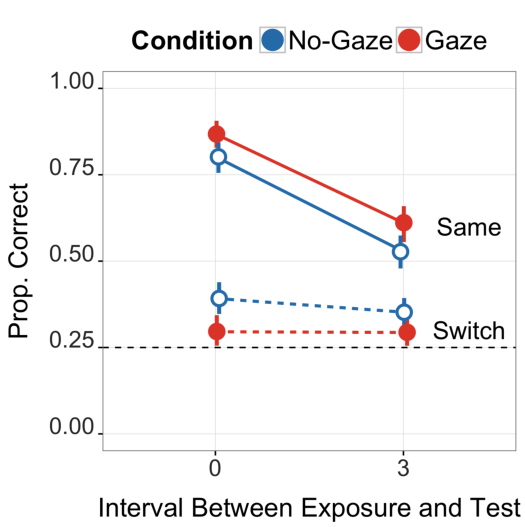
\includegraphics[width=0.5\linewidth]{figs/expt4-plot-1} 

}

\caption[Experiment 4 results]{\DIFaddFL{Experiment 4 results. Accuracy on test trials in Experiment 4 collapsed across the Long and Short inspection time conditions. The dashed line represents chance performance. Color and line type indicate whether there was gaze present on exposure trials. Error bars indicate 95\% confidence intervals computed by non-parametric bootstrap. }}\label{fig:expt4-plot}
\end{figure}
\end{CodeChunk}

\subsection{\DIFadd{Method}}\label{method-3}

\subsubsection{\DIFadd{Participants}}\label{participants-3}

\DIFadd{Participant recruitment and inclusionary/exclusionary criteria were
identical to those of Experiments 1, 2, and 3. 100 HITs were posted for
each condition (1 Referent X 2 Intervals X 2 Inspection Time conditions)
for total of 400 paid HITs (excluded 37 HITs).
}

\subsubsection{\DIFadd{Stimuli}}\label{stimuli-2}

\DIFadd{Audio, picture, and video stimuli were identical to Experiments 2 and 3.
Since inspection times were fixed across conditions, we wanted to ensure
that participants were aware of the time remaining on each exposure
trial. So we included a circular countdown timer located above the
center video. The timer remained on the screen during test trials but
did not count down since participants could take as much time as they
wanted to respond on test trials.
}

\subsubsection{\DIFadd{Design and Procedure}}\label{design-and-procedure-3}

\DIFadd{Procedures were identical to those of Experiment 1-3. The design was
identical to that of Experiment 2 and consisted of 32 trials split into
2 blocks of 16 trials. Each block consisted of 8 exposure trials and 8
test trials (4 Same trials and 4 Switch trials) and contained only Gaze
or No-Gaze exposure trials. The order of block was counterbalanced
across participants.
}

\DIFadd{The major design change was to make the length of exposure trials
equivalent across the Gaze and No-Gaze conditions. We randomly assigned
participants to one of two inspection time conditions: Short (6 seconds)
or Long (9 seconds). These times were selected based on participants'
self-paced inspection times in the Gaze and No-Gaze conditions in
Experiment 2. After pilot testing, we added three seconds to each
condition to ensure that participants had enough time to respond before
the experiment advanced. If participants did not respond in the allotted
time, an error message appeared informing participants that time had run
out and encouraged them to respond within the time window on subsequent
trials.
}

\subsection{\DIFadd{Results and Discussion}}\label{results-and-discussion-3}

\DIFadd{We did not see strong evidence of an effect of the different inspection
times. Thus, all of the results reported here collapse across the short
and long inspection time conditions. For all analyses, we removed the
trials on which participants did not respond within the fixed inspection
time on exposure trials (0.05\% of trials).
}

\subsubsection{\DIFadd{Exposure Trials}}\label{exposure-trials-3}

\DIFadd{Participants' responses on exposure trials differed from those expected
by chance (smallest \(\beta\) = 2.95, z = 38.08, \(p\) \textless{}
.001), suggesting that gaze was again effective in directing
participants' attention. Similar to Experiment 2, participants were
quite likely to use the gaze cue when it was a live actress
(\(M_{0-interval}\) = 0.93, \(M_{3-interval}\) = 0.95).
}

\subsubsection{\DIFadd{Test Trials}}\label{test-trials-3}

\DIFadd{Figure 6 shows performance on test trials in Experiment 4. In the
majority of conditions, participants selected the correct referent at
rates greater than chance (smallest \(\beta\) = 0.2, z = 2.2, \(p\)
\textless{} .05). However, participants' responses were only marginally
different from chance on Switch trials after exposure trials with gaze
in the 3-interval condition (\(\beta\) = 0.17, \(p\) = 0.06).
}

\DIFadd{We replicate the key finding from Experiments 1-3: after seeing exposure
trials with gaze, participants were less accurate on Switch trials
(\(\beta\) = 0.9, \(p\) \textless{} .001). Since inspection times were
fixed across the Gaze and No-Gaze conditions, this finding provides
evidence that the presence of a referential cue did more than just
reduce the amount of time participants' spent inspecting the potential
word-object links. In contrast to Experiments 1-3, visual inspection of
Figure 6 suggested that the referential cue provided a boost to accuracy
on Same trials. To assess the simple effects of gaze on trial type, we
computed pairwise contrasts using the }\emph{\DIFadd{lsmeans}} \DIFadd{package in R with a
Bonferroni correction for multiple comparisons (Lenth, 2016). Accuracy
was higher for Same trials in the Gaze condition (\(\beta\) = 0.49,
\(p\) \textless{} .001), but lower for Switch trials (\(\beta\) = -0.41,
\(p\) \textless{} .001). The boost in accuracy on Same trials differs
from Experiments 1-3 and suggests that making inspection times
equivalent across conditions allowed the social cue to affect the
strength of learners' memory for their candidate hypothesis.
}

\DIFadd{The results of Experiment 4 help to clarify the effect of gaze on memory
in our task, providing evidence that the presence of a referential cue
did more than just reduce participants' visual inspection time. Instead,
gaze reduced memory for alternative word-object links even when people
had the same opportunity to visually inspect and encode the word-object
links. We also found evidence of a boost for learners' memory of their
candidate hypothesis in the gaze condition, an effect that we did not
see in Experiments 1-3. One explanation for this difference is that in
Experiment 4 since participants' use of gaze was independent of the
length of exposure trials, inspection times in the gaze condition were
longer compared to those in Experiments 1-3. Thus, it could be that the
combination of a gaze cue with the opportunity to continue attending to
the gaze target led to a boost in performance on Same trials relative to
trials without gaze.
}

\DIFaddend \section{General Discussion}\label{general-discussion}

Tracking cross-situational word-object statistics allows word learning
to proceed despite the presence of individually ambiguous naming events.
But models of cross-situational learning disagree about how much
information is actually stored in memory\DIFdelbegin \DIFdel{and how to best characterize
}\DIFdelend \DIFaddbegin \DIFadd{, and }\DIFaddend the input to statistical
learning mechanisms \DIFaddbegin \DIFadd{can vary along a continuum of referential
uncertainty}\DIFaddend . In the current line of work, we explore the hypothesis that
these two factors are fundamentally linked \DIFdelbegin \DIFdel{, both }\DIFdelend to one another and to the
social context in which word learning occurs. Specifically, we ask how
cross-situational learning operates over social input that \DIFdelbegin \DIFdel{varies along a continuum from low to
high ambiguity }\DIFdelend \DIFaddbegin \DIFadd{modulates the
amount of ambiguity in the each learning context}\DIFaddend .

Our results suggest that the representations underlying
cross-situational learning are quite flexible. In the absence of a
referential cue to word meaning, \DIFdelbegin \DIFdel{learners were more likely to store }\DIFdelend \DIFaddbegin \DIFadd{people tended to store more }\DIFaddend alternative
word-object links. In contrast, when gaze was present \DIFdelbegin \DIFdel{, they
}\DIFdelend \DIFaddbegin \DIFadd{learners }\DIFaddend stored
less information, showing behavior consistent with tracking a single
hypothesis (Experiments 1 and 2). Learners were also sensitive to a
parametric manipulation of the \DIFaddbegin \DIFadd{strength of the }\DIFaddend referential cue, showing
a graded increase in the tendency to use the cue as reliability
increased, which in turn resulted in a graded decrease in memory for
alternative word-object links (Experiment 3). \DIFdelbegin \DIFdel{Across all three experiments, }\DIFdelend \DIFaddbegin \DIFadd{Finally, learners stored
less information in the presence of gaze even when they spent the same
amount of time visually inspecting the objects during learning
(Experiment 4).
}

\DIFadd{In Experiments 1-3, }\DIFaddend reduced memory for alternative hypotheses did not
result in a boost \DIFdelbegin \DIFdel{in }\DIFdelend \DIFaddbegin \DIFadd{to }\DIFaddend memory for learners' candidate hypothesis. This
pattern of data suggests that the presence of a referential cue
selectively affected one component of the underlying representation: the
number of alternative word-object links, and not learners\DIFaddbegin \DIFadd{' }\DIFaddend candidate
hypothesis. \DIFaddbegin \DIFadd{However, when the length of exposure trials was equivalent
across the gaze and no-gaze conditions in Experiment 4, learners showed
stronger memory for their initial hypothesis when gaze was present. This
suggests that the relationship between referential cues and the strength
of learners' candidate hypothesis is modulated by how the cue interacts
with attention: When coupled with the opportunity for sustained
attention, gaze provided a boost to memory.
}\DIFaddend 

\subsection{Relationship to previous
work}\label{relationship-to-previous-work}

Why \DIFdelbegin \DIFdel{did we not see an increase in }\DIFdelend \DIFaddbegin \DIFadd{else would a decrease in memory for alternatives fail to increase
}\DIFaddend the strength of learners' \DIFaddbegin \DIFadd{memory for their }\DIFaddend candidate hypothesis? One
possibility is that \DIFdelbegin \DIFdel{participants }\DIFdelend \DIFaddbegin \DIFadd{people }\DIFaddend did not shift their cognitive resources from
the set of alternatives to their single hypothesis, but instead \DIFdelbegin \DIFdel{rationally conserved }\DIFdelend \DIFaddbegin \DIFadd{chose to
conserve }\DIFaddend their resources for future use. Griffiths, Lieder, \DIFdelbegin \DIFdel{\& }\DIFdelend \DIFaddbegin \DIFadd{and }\DIFaddend Goodman
(2015) formalize this behavior by pushing the rationality of
computational-level models down to the psychological process level. In
their framework, cognitive systems are thought to be adaptive in that
they optimize the use of their limited resources, taking the cost of
computation (e.g., \DIFaddbegin \DIFadd{the }\DIFaddend opportunity cost of time or mental \DIFdelbegin \DIFdel{opportunity}\DIFdelend \DIFaddbegin \DIFadd{energy}\DIFaddend ) into
account. For example, Vul, Goodman, Griffiths, \DIFdelbegin \DIFdel{\& }\DIFdelend \DIFaddbegin \DIFadd{and }\DIFaddend Tenenbaum (2014)
showed that as time pressure increased in a decision-making task,
participants were more likely to show behavior consistent with a less
cognitively challenging strategy of matching, rather than with the
globally optimal strategy. In the current work, we found that learners
showed evidence of \DIFdelbegin \DIFdel{changing }\DIFdelend \DIFaddbegin \DIFadd{altering }\DIFaddend how they allocated cognitive resources based
on the amount of referential uncertainty \DIFaddbegin \DIFadd{present during learning}\DIFaddend ,
spending less time \DIFdelbegin \DIFdel{studying }\DIFdelend \DIFaddbegin \DIFadd{inspecting }\DIFaddend alternative word-object links and reducing
the number of links stored in memory when uncertainty was low.

Our results also fit well with recent experimental work that
investigates how attention and memory can constrain infants' statistical
word learning. For example, \DIFdelbegin \DIFdel{L. B. Smith \& }\DIFdelend \DIFaddbegin \DIFadd{Smith and }\DIFaddend Yu (2013) used a modified
cross-situational learning task to show that only infants who disengaged
from a novel object to look at both potential referents were able to
learn the correct word--object mappings. Moreover, Vlach \DIFdelbegin \DIFdel{\& }\DIFdelend \DIFaddbegin \DIFadd{and }\DIFaddend Johnson
(2013) showed that 16-month-olds were only able to learn from adjacent
cross-situational co-occurrence statistics, and unable to learn from
co-occurrences that were separated in time. Both of these findings make
the important point that only the information that comes into contact
with the learning system can be used for cross-situational word
learning, and this information is directly influenced by the attention
and memory constraints of the learner.
\DIFaddbegin 

\DIFadd{Moreover, these results add to a large literature showing the importance
of social information for word learning (P. Bloom, 2002; Clark, 2009)
and exploring the interaction between statistical learning and other
types of information (Frank, Goodman, \& Tenenbaum, 2009; Koehne \&
Crocker, 2014; Yu \& Ballard, 2007). For example, Yoshida, Rhemtulla,
and Vouloumanos (2012) showed that in an statistical learning task
adults only used exclusion learning processes (i.e., discarding known
alternatives) with speech stimuli, and not for nonspeech labels,
suggesting that statistical learning operated differently depending on
the nature of the input. }\DIFaddend Our findings suggest that referential cues
\DIFdelbegin \DIFdel{could play an
important role in constraining the input
to statistical learning mechanisms}\DIFdelend \DIFaddbegin \DIFadd{interact with statistical learning by modulating the amount of
information that people store in the underlying representations that
support learning over time.
}

\DIFadd{Is gaze a privileged cue, or could other, less-social cues (e.g., an
arrow) also affect the representations underlying cross-situational
learning? On the one hand, previous research has shown that gaze cues
lead to more reflexive attentional responses compared to arrows
(Friesen, Ristic, \& Kingstone, 2004), that gaze-triggered attention
results in better learning compared to salience-triggered attention (Wu
\& Kirkham, 2010), and that even toddlers readily use gaze to infer
novel word meanings (Baldwin, 1993). Thus, it could be that gaze is an
especially effective cue for constraining word learning since it
communicates a speaker's referential intent and is a particularly good
way to guide attention. On the other hand, the generative process of the
cue -- whether it is more or less social in nature -- might be less
important; instead, the critical factor might be whether the cue
effectively reduces uncertainty in the naming event. Under this account,
gaze is placed amongst a set of many cues that could produce similar
effects as those reported here. Future work could explore a wider range
of cues to see if they modulate the representations underlying
cross-situational learning in a similar way}\DIFaddend .

\DIFdelbegin \DIFdel{How }\DIFdelend \DIFaddbegin \DIFadd{But how }\DIFaddend should we characterize the effect of \DIFdelbegin \DIFdel{social information }\DIFdelend \DIFaddbegin \DIFadd{gaze }\DIFaddend on attention and
memory in our task? One possibility is that the referential cue acts as
a filter, only allowing likely referents to contact statistical learning
mechanisms (Yu \& Ballard, 2007). This `filtering account' separates the
effect of social cues from the underlying computation that aggregates
cross-situational information. Another possibility is that referential
cues provide evidence about a speaker's communicative intent (Frank \DIFdelbegin \DIFdel{, Goodman, \& Tenenbaum, }\DIFdelend \DIFaddbegin \DIFadd{et
al., }\DIFaddend 2009). In this model, the learner is reasoning about the speaker
and word meanings simultaneously, which places inferences based on
social information as part of the underlying computation. A third
possibility is that participants thought of the referential cue as
pedagogical. In this \DIFdelbegin \DIFdel{scenario}\DIFdelend \DIFaddbegin \DIFadd{context}\DIFaddend , learners assume that the speaker will
choose an action that is most likely to increase the learner's belief in
the true state of the world (Shafto, Goodman, \& Frank, 2012), making it
unnecessary to allocate resources to alternative hypotheses. Experiments
show that children spend less time exploring an object and are less
likely to discover alternative object-functions \DIFdelbegin \DIFdel{, }\DIFdelend if a single function is
demonstrated in a pedagogical context (Bonawitz et al., 2011). However,
because the results from the current study cannot distinguish between
these explanations, these questions remain topics for future studies
specifically designed to tease apart these possibilities.

\subsection{Limitations}\label{limitations}

There are several limitations to the current study that are worth
noting. First, the social context \DIFaddbegin \DIFadd{that }\DIFaddend we used was relatively
impoverished. Although we moved beyond a simple manipulation of the
presence or absence of social information, we isolated just a single cue
to reference, gaze. But real-world learning contexts are much more
complex, providing learners access to multiple cues such as gaze,
pointing, and previous discourse. In fact, Frank, Tenenbaum, \DIFdelbegin \DIFdel{\& }\DIFdelend \DIFaddbegin \DIFadd{and }\DIFaddend Fernald
(2013) analyzed a corpus of parent-child interactions and concluded that
learners would do better to aggregate noisy social information from
multiple cues, rather than monitor a single cue \DIFdelbegin \DIFdel{, because }\DIFdelend \DIFaddbegin \DIFadd{since }\DIFaddend no single cue was
a consistent predictor of reference\DIFdelbegin \DIFdel{in their corpus}\DIFdelend . In our data, we did see a more
reliable effect of referential cues when we used a live actress, which
included both gaze and head turn as opposed to the static, schematic
stimuli, which only included gaze. It is still an open and interesting
question as to how our results would generalize to \DIFdelbegin \DIFdel{real-world }\DIFdelend learning environments
that contain a rich combination of social cues.

Second, we do not yet know how \DIFdelbegin \DIFdel{these results would generalize to }\DIFdelend \DIFaddbegin \DIFadd{variations in referential uncertainty
during learning would affect the representations of }\DIFaddend young word learners\DIFdelbegin \DIFdel{. Research with infants'shows rapid development of visual
}\DIFdelend \DIFaddbegin \DIFadd{,
the age at which cross-situational word learning might be particularly
important. Recent research using a similar paradigm as our own did not
find evidence that 2- or 3-year-olds stored multiple word-object links;
instead, children only retained a single candidate hypothesis (Woodard,
Gleitman, \& Trueswell, 2016). However, performance limitations on
children's developing }\DIFaddend attention and memory \DIFdelbegin \DIFdel{in the first years of life }\DIFdelend \DIFaddbegin \DIFadd{systems }\DIFaddend (Colombo, 2001;
Ross-sheehy, Oakes, \& Luck, 2003) \DIFdelbegin \DIFdel{. Moreover, experimental work shows
that infants ' }\DIFdelend \DIFaddbegin \DIFadd{could make success on these explicit
response tasks more difficult. Thus, we think that it will be important
to test a variety of outcome measures to see if younger learners show
evidence of storing multiple word meanings during learning.
}

\DIFadd{Moreover, previous work with infants has shown that their }\DIFaddend attention is
often \DIFdelbegin \DIFdel{stimulus driven }\DIFdelend \DIFaddbegin \DIFadd{stimulus-driven }\DIFaddend and sticky (Oakes, 2011), suggesting that very
young word learners might not effectively explore the visual scene \DIFaddbegin \DIFadd{in
order }\DIFaddend to extract the necessary statistics for \DIFdelbegin \DIFdel{effective cross-situational word learning. The current work suggests
}\DIFdelend \DIFaddbegin \DIFadd{storing multiple
alternatives. It could be }\DIFaddend that referential cues \DIFdelbegin \DIFdel{might }\DIFdelend play an even more
important role for young learners \DIFdelbegin \DIFdel{, guiding them }\DIFdelend \DIFaddbegin \DIFadd{by filtering the input to
cross-situational word learning mechanisms and guiding children }\DIFaddend to the
relevant statistics in the input. \DIFaddbegin \DIFadd{In fact, recent work has shown that
the precise timing of features such as increased parent attention and
gesturing towards a named object and away from non-target objects were
strong predictors of referential clarity in a naming event (Trueswell et
al., 2016). It could be that the statistics available in these
particularly unambiguous naming events are the most useful for
cross-situational learning.
}\DIFaddend 

\DIFdelbegin \DIFdel{And third, in the current experiments we tested a minimal
}\DIFdelend \DIFaddbegin \DIFadd{Finally, the current experiments used a restricted }\DIFaddend cross-situational
\DIFdelbegin \DIFdel{learning scenario. Our task contained only one
}\DIFdelend \DIFaddbegin \DIFadd{word learning scenario, which differs from real-world language learning
contexts in several important ways. One, we only tested a single
}\DIFaddend exposure for each novel word-object pairing\DIFdelbegin \DIFdel{. In contrast, real world
}\DIFdelend \DIFaddbegin \DIFadd{; whereas, real-world }\DIFaddend naming
events are best characterized by discourse \DIFdelbegin \DIFdel{, }\DIFdelend where an object is likely to
be named repeatedly in a short amount of time (Frank\DIFdelbegin \DIFdel{et al., }\DIFdelend \DIFaddbegin \DIFadd{, Tenenbaum, \&
Fernald, }\DIFaddend 2013; Rohde \& Frank, 2014). \DIFdelbegin \DIFdel{Moreover, }\DIFdelend \DIFaddbegin \DIFadd{Two, the restricted visual world
of 2-8 objects on a screen combined with the forced-choice response
format may have biased people to assume that all words in the task must
have referred to one of the objects. But, in actual language use, people
can refer to things that are not physically co-present (e.g., L.
Gleitman, 1990), creating a scenario where learners would not benefit
from storing additional word-object links in the absence of clear
referential cues. Finally, }\DIFaddend we presented novel words in isolation,
removing any sentential cues to word meaning (e.g., verb-argument
relations). \DIFdelbegin \DIFdel{Previous work shows that sentence-level
constraints do interact with }\DIFdelend \DIFaddbegin \DIFadd{In fact, previous work with adults has shown that
}\DIFaddend cross-situational \DIFdelbegin \DIFdel{word learning mechanisms }\DIFdelend \DIFaddbegin \DIFadd{learning mechanisms only operate in contexts where
sentence-level constraints do not completely disambiguate meaning
}\DIFaddend (Koehne \& Crocker, 2014). \DIFdelbegin \DIFdel{We }\DIFdelend \DIFaddbegin \DIFadd{Thus, we }\DIFaddend need more evidence to understand how
\DIFaddbegin \DIFadd{the }\DIFaddend representations underlying cross-situational learning change in
response to referential uncertainty at different timescales and in
richer language contexts that more accurately reflect \DIFaddbegin \DIFadd{real-world
}\DIFaddend learning environments.

\subsection{Conclusions}\label{conclusions}

Word learning proceeds despite the potential for high levels of
referential uncertainty and \DIFaddbegin \DIFadd{despite }\DIFaddend learners' limited cognitive
resources. Our work shows that cross-situational learners flexibly
respond to the amount of ambiguity in the input, and as referential
uncertainty increases, learners \DIFaddbegin \DIFadd{tended to }\DIFaddend store more word-object links.
Overall, these results bring together aspects of \DIFdelbegin \DIFdel{both }\DIFdelend social and statistical
accounts of word learning \DIFdelbegin \DIFdel{, and }\DIFdelend \DIFaddbegin \DIFadd{to }\DIFaddend increase our understanding of how \DIFaddbegin \DIFadd{social
information modulates the input to }\DIFaddend statistical learning mechanisms\DIFdelbegin \DIFdel{operate over fundamentally social input}\DIFdelend .

\newpage

\section{Acknowledgements}\label{acknowledgements}

We are grateful to Rose Schneider for helping record stimuli and to the
members of the Language and Cognition Lab for their feedback on this
project\DIFaddbegin \DIFadd{. }\DIFaddend This work was supported by a National Science Foundation
Graduate Research Fellowship to KM, an NIH NRSA Postdoctoral Fellowship
to DY, and a John Merck Scholars Fellowship to M.C.F.

\newpage

\DIFdelbegin \section*{\DIFdel{References}}%DIFAUXCMD
\DIFdelend \DIFaddbegin \section{\DIFadd{References}}\DIFaddend \label{references}
\DIFdelbegin \addcontentsline{toc}{section}{\DIFdel{References}}
%DIFAUXCMD
\DIFdelend 

\DIFaddbegin \setlength{\parindent}{-0.1in} \setlength{\leftskip}{0.125in} \noindent

\hypertarget{refs}{}
\hypertarget{ref-baldwin1993infants}{}
\DIFaddend Baldwin, D. A. (1993). Infants' ability to consult the speaker for clues
to word reference. \emph{Journal of Child Language}, \emph{20}(02),
395--418.

\DIFaddbegin \hypertarget{ref-bates2013lme4}{}
\DIFaddend Bates, D., Maechler, M., Bolker, B., \& Walker, S. (2013). Lme4: Linear
mixed-effects models using eigen and s4. \emph{R Package Version},
\emph{1}(4).

\DIFaddbegin \hypertarget{ref-bloom2002children}{}
\DIFaddend Bloom, P. (2002). \emph{How children learn the meaning of words}. The
MIT Press.

\DIFaddbegin \hypertarget{ref-bonawitz2011double}{}
\DIFaddend Bonawitz, E., Shafto, P., Gweon, H., Goodman, N. D., Spelke, E., \&
Schulz, L. (2011). The double-edged sword of pedagogy: Instruction
limits spontaneous exploration and discovery. \emph{Cognition},
\emph{120}(3), 322--330.

\DIFaddbegin \hypertarget{ref-brooks2005development}{}
\DIFaddend Brooks, R., \& Meltzoff, A. N. (2005). The development of gaze following
and its relation to language. \emph{Developmental Science}, \emph{8}(6),
535--543.

\DIFaddbegin \hypertarget{ref-brooks2008infant}{}
\DIFaddend Brooks, R., \& Meltzoff, A. N. (2008). Infant gaze following and
pointing predict accelerated vocabulary growth through two years of age:
A longitudinal, growth curve modeling study. \emph{Journal of Child
Language}, \emph{35}(01), 207--220.

\DIFaddbegin \hypertarget{ref-carpenter1998social}{}
\DIFaddend Carpenter, M., Nagell, K., Tomasello, M., Butterworth, G., \& Moore, C.
(1998). Social cognition, joint attention, and communicative competence
from 9 to 15 months of age. \emph{Monographs of the Society for Research
in Child Development}, i--174.

\DIFaddbegin \hypertarget{ref-cartmill2013quality}{}
\DIFaddend Cartmill, E. A., Armstrong, B. F., Gleitman, L. R., Goldin-Meadow, S.,
Medina, T. N., \& Trueswell, J. C. (2013). Quality of early parent input
predicts child vocabulary 3 years later. \emph{Proceedings of the
National Academy of Sciences}, \emph{110}(28), 11278--11283.

\DIFaddbegin \hypertarget{ref-clark2009first}{}
\DIFaddend Clark, E. V. (2009). \emph{First language acquisition}. Cambridge
University Press.

\DIFaddbegin \hypertarget{ref-cleveland2007joint}{}
\DIFaddend Cleveland, A., Schug, M., \& Striano, T. (2007). Joint attention and
object learning in 5-and 7-month-old infants. \emph{Infant and Child
Development}, \emph{16}(3), 295--306.

\DIFaddbegin \hypertarget{ref-colombo2001development}{}
\DIFaddend Colombo, J. (2001). The development of visual attention in infancy.
\emph{Annual Review of Psychology}, \emph{52}(1), 337--367.

\DIFaddbegin \hypertarget{ref-frank2009using}{}
\DIFaddend Frank, M. C., Goodman, N. D., \& Tenenbaum, J. B. (2009). Using
speakers' referential intentions to model early cross-situational word
learning. \emph{Psychological Science}, \emph{20}(5), 578--585.

\DIFaddbegin \hypertarget{ref-frank2013social}{}
\DIFaddend Frank, M. C., Tenenbaum, J. B., \& Fernald, A. (2013). Social and
discourse contributions to the determination of reference in
cross-situational word learning. \emph{Language Learning and
Development}, \emph{9}(1), 1--24.

\DIFaddbegin \hypertarget{ref-friesen2004attentional}{}
\DIFadd{Friesen, C. K., Ristic, J., \& Kingstone, A. (2004). Attentional effects
of counterpredictive gaze and arrow cues. }\emph{\DIFadd{Journal of Experimental
Psychology: Human Perception and Performance}}\DIFadd{, }\emph{30}(2)\DIFadd{, 319.
}

\hypertarget{ref-gillette1999human}{}
\DIFadd{Gillette, J., Gleitman, H., Gleitman, L., \& Lederer, A. (1999). Human
simulations of vocabulary learning. }\emph{\DIFadd{Cognition}}\DIFadd{, }\emph{73}(2)\DIFadd{,
135--176.
}

\hypertarget{ref-gleitman1990structural}{}
\DIFadd{Gleitman, L. (1990). The structural sources of verb meanings.
}\emph{\DIFadd{Language Acquisition}}\DIFadd{, }\emph{1}(1)\DIFadd{, 3--55.
}

\hypertarget{ref-griffiths2015rational}{}
\DIFaddend Griffiths, T. L., Lieder, F., \& Goodman, N. D. (2015). Rational use of
cognitive resources: Levels of analysis between the computational and
the algorithmic. \emph{Topics in Cognitive Science}, \emph{7}(2),
217--229.

\DIFaddbegin \hypertarget{ref-hollich2000breaking}{}
\DIFaddend Hollich, G. J., Hirsh-Pasek, K., Golinkoff, R. M., Brand, R. J., Brown,
E., Chung, H. L., \ldots{} Bloom, L. (2000). Breaking the language
barrier: An emergentist coalition model for the origins of word
learning. \emph{Monographs of the Society for Research in Child
Development}, i--135.

\DIFaddbegin \hypertarget{ref-kanwisher1997locus}{}
\DIFaddend Kanwisher, N., Woods, R. P., Iacoboni, M., \& Mazziotta, J. C. (1997). A
locus in human extrastriate cortex for visual shape analysis.
\emph{Journal of Cognitive Neuroscience}, \emph{9}(1), 133--142.

\DIFaddbegin \hypertarget{ref-koehne2014interplay}{}
\DIFaddend Koehne, J., \& Crocker, M. W. (2014). The interplay of cross-situational
word learning and sentence-level constraints. \emph{Cognitive Science}.

\DIFaddbegin \hypertarget{ref-koenig2004trust}{}
\DIFaddend Koenig, M. A., Clement, F., \& Harris, P. L. (2004). Trust in testimony:
Children's use of true and false statements. \emph{Psychological
Science}, \emph{15}(10), 694--698.

\DIFaddbegin \hypertarget{ref-lenth2016lsmeans}{}
\DIFadd{Lenth, R. V. (2016). Least-squares means: The R package lsmeans.
}\emph{\DIFadd{Journal of Statistical Software}}\DIFadd{, }\emph{69}(1)\DIFadd{, 1--33.
}\url{http://doi.org/10.18637/jss.v069.i01}

\hypertarget{ref-mcmurray2012word}{}
\DIFaddend McMurray, B., Horst, J. S., \& Samuelson, L. K. (2012). Word learning
emerges from the interaction of online referent selection and slow
associative learning. \emph{Psychological Review}, \emph{119}(4), 831.

\DIFaddbegin \hypertarget{ref-medina2011words}{}
\DIFaddend Medina, T. N., Snedeker, J., Trueswell, J. C., \& Gleitman, L. R.
(2011). How words can and cannot be learned by observation.
\emph{Proceedings of the National Academy of Sciences}, \emph{108}(22),
9014--9019.

\DIFaddbegin \hypertarget{ref-oakes2011infant}{}
\DIFaddend Oakes, L. M. (2011). \emph{Infant perception and cognition: Recent
advances, emerging theories, and future directions}. Oxford University
Press, USA.

\DIFaddbegin \hypertarget{ref-quine19600}{}
\DIFaddend Quine, W. V. (1960). 0. word and object. \emph{111e MIT Press}.

\DIFaddbegin \hypertarget{ref-rohde2014markers}{}
\DIFaddend Rohde, H., \& Frank, M. C. (2014). Markers of topical discourse in
child-directed speech. \emph{Cognitive Science}, \emph{38}(8),
1634--1661.

\DIFaddbegin \hypertarget{ref-ross2003development}{}
\DIFaddend Ross-sheehy, S., Oakes, L. M., \& Luck, S. J. (2003). The development of
visual short-term memory capacity in infants. \emph{Child Development},
\emph{74}(6), 1807--1822.

\DIFaddbegin \hypertarget{ref-shafto2012learning}{}
\DIFaddend Shafto, P., Goodman, N. D., \& Frank, M. C. (2012). Learning from others
the consequences of psychological reasoning for human learning.
\emph{Perspectives on Psychological Science}, \emph{7}(4), 341--351.

\DIFaddbegin \hypertarget{ref-siskind1996computational}{}
\DIFaddend Siskind, J. M. (1996). A computational study of cross-situational
techniques for learning word-to-meaning mappings. \emph{Cognition},
\emph{61}(1), 39--91.

\DIFaddbegin \hypertarget{ref-smith2011cross}{}
\DIFaddend Smith, K., Smith, A. D., \& Blythe, R. A. (2011). Cross-situational
learning: An experimental study of word-learning mechanisms.
\emph{Cognitive Science}, \emph{35}(3), 480--498.

\DIFaddbegin \hypertarget{ref-smith2008infants}{}
\DIFaddend Smith, L. B., \& Yu, C. (\DIFaddbegin \DIFadd{2008). Infants rapidly learn word-referent
mappings via cross-situational statistics. }\emph{\DIFadd{Cognition}}\DIFadd{,
}\emph{106}(3)\DIFadd{, 1558--1568.
}

\hypertarget{ref-smith2013visual}{}
\DIFadd{Smith, L. B., \& Yu, C. (}\DIFaddend 2013). Visual attention is not enough:
Individual differences in statistical word-referent learning in infants.
\emph{Language Learning and Development}, \emph{9}(1), 25--49.

\DIFaddbegin \hypertarget{ref-smith2014unrealized}{}
\DIFaddend Smith, L. B., Suanda, S. H., \& Yu, C. (2014). The unrealized promise of
infant statistical word--referent learning. \emph{Trends in Cognitive
Sciences}, \emph{18}(5), 251--258.

\DIFdelbegin \DIFdel{Smith, }\DIFdelend \DIFaddbegin \hypertarget{ref-trueswell2016perceiving}{}
\DIFadd{Trueswell, J. C., Lin, Y., Armstrong, B., Cartmill, E. A.,
Goldin-Meadow, S., \& Gleitman, }\DIFaddend L. \DIFdelbegin \DIFdel{, \& Yu, C. (2008). Infants rapidly learn word-referent
mappings via cross-situational statistics}\DIFdelend \DIFaddbegin \DIFadd{R. (2016). Perceiving referential
intent: Dynamics of reference in natural parent--child interactions}\DIFaddend .
\emph{Cognition}, \DIFdelbegin %DIFDELCMD < \emph{106}(3)%%%
\DIFdel{, 1558--1568}\DIFdelend \DIFaddbegin \emph{\DIFadd{148}}\DIFadd{, 117--135}\DIFaddend .

\DIFaddbegin \hypertarget{ref-trueswell2013propose}{}
\DIFaddend Trueswell, J. C., Medina, T. N., Hafri, A., \& Gleitman, L. R. (2013).
Propose but verify: Fast mapping meets cross-situational word learning.
\emph{Cognitive Psychology}, \emph{66}(1), 126--156.

\DIFaddbegin \hypertarget{ref-vlach2013memory}{}
\DIFaddend Vlach, H. A., \& Johnson, S. P. (2013). Memory constraints on infants'
cross-situational statistical learning. \emph{Cognition}, \emph{127}(3),
375--382.

\DIFaddbegin \hypertarget{ref-vouloumanos2008fine}{}
\DIFaddend Vouloumanos, A. (2008). Fine-grained sensitivity to statistical
information in adult word learning. \emph{Cognition}, \emph{107}(2),
729--742.

\DIFaddbegin \hypertarget{ref-vul2014}{}
\DIFaddend Vul, E., Goodman, N., Griffiths, T. L., \& Tenenbaum, J. B. (2014). One
and done? Optimal decisions from very few samples. \emph{Cognitive
Science}, \emph{38}(4), 599--637.

\DIFaddbegin \hypertarget{ref-woodard2016two}{}
\DIFadd{Woodard, K., Gleitman, L. R., \& Trueswell, J. C. (2016). Two-and
three-year-olds track a single meaning during word learning: Evidence
for propose-but-verify. }\emph{\DIFadd{Language Learning and Development}}\DIFadd{,
}\emph{12}(3)\DIFadd{, 252--261.
}

\hypertarget{ref-wu2010no}{}
\DIFaddend Wu, R., \DIFaddbegin \DIFadd{\& Kirkham, N. Z. (2010). No two cues are alike: Depth of
learning during infancy is dependent on what orients attention.
}\emph{\DIFadd{Journal of Experimental Child Psychology}}\DIFadd{, }\emph{107}(2)\DIFadd{,
118--136.
}

\hypertarget{ref-wu2011infants}{}
\DIFadd{Wu, R., }\DIFaddend Gopnik, A., Richardson, D. C., \& Kirkham, N. Z. (2011). Infants
learn about objects from statistics and people. \emph{Developmental
Psychology}, \emph{47}(5), 1220.

\DIFaddbegin \hypertarget{ref-yoon2008communication}{}
\DIFaddend Yoon, J. M., Johnson, M. H., \& Csibra, G. (2008). Communication-induced
memory biases in preverbal infants. \emph{Proceedings of the National
Academy of Sciences}, \emph{105}(36), 13690--13695.

\DIFaddbegin \hypertarget{ref-yoshida2012exclusion}{}
\DIFadd{Yoshida, K., Rhemtulla, M., \& Vouloumanos, A. (2012). Exclusion
constraints facilitate statistical word learning. }\emph{\DIFadd{Cognitive
Science}}\DIFadd{, }\emph{36}(5)\DIFadd{, 933--947.
}

\hypertarget{ref-yu2007unified}{}
\DIFaddend Yu, C., \& Ballard, D. H. (2007). A unified model of early word
learning: Integrating statistical and social cues.
\emph{Neurocomputing}, \emph{70}(13), 2149--2165.

\DIFaddbegin \hypertarget{ref-yu2007rapid}{}
\DIFaddend Yu, C., \& Smith, L. B. (2007). Rapid word learning under uncertainty
via cross-situational statistics. \emph{Psychological Science},
\emph{18}(5), 414--420.

\DIFaddbegin \hypertarget{ref-yu2012embodied}{}
\DIFaddend Yu, C., \& Smith, L. B. (2012). Embodied attention and word learning by
toddlers. \emph{Cognition}.

\DIFaddbegin \hypertarget{ref-yurovsky2014algorithmic}{}
\DIFaddend Yurovsky, D., \& Frank, M. C. (2015). An integrative account of
constraints on cross-situational learning. \emph{Cognition}.

\DIFaddbegin \hypertarget{ref-yurovsky2013statistical}{}
\DIFaddend Yurovsky, D., Smith, L. B., \& Yu, C. (2013). Statistical word learning
at scale: The baby's view is better. \emph{Developmental Science},
\emph{16}(6), 959--966.

\bibliography{}

\end{document}
